\documentclass[letterpaper]{article}
\usepackage{uai2020}
\usepackage[margin=1in]{geometry}
\usepackage{times}

\usepackage[ruled,vlined]{algorithm2e}
\usepackage{amssymb}
\usepackage{mathtools}
\usepackage[capitalise]{cleveref}
\usepackage{tikz}
\usepackage{mathrsfs}
\usepackage[nounderscore]{syntax}
\usepackage{blkarray}
\usepackage{siunitx}
\usepackage{amsthm}
\usepackage[round]{natbib}
\usepackage[inline]{enumitem}

\newtheorem{constraint}{Constraint}
\theoremstyle{definition}
\newtheorem{definition}{Definition}
\newtheorem{example}{Example}

\renewcommand\fbox{\fcolorbox{red}{white}}

\makeatletter
\newcommand{\nosemic}{\renewcommand{\@endalgocfline}{\relax}}% Drop semi-colon ;
\newcommand{\dosemic}{\renewcommand{\@endalgocfline}{\algocf@endline}}% Reinstate semi-colon ;
\newcommand{\pushline}{\Indp}% Indent
\newcommand{\popline}{\Indm\dosemic}% Undent
\makeatother

\newcommand{\logical}[1]{{\normalfont \texttt{#1}}}
\newcommand{\variable}[1]{\texttt{\textup{#1}}}
\newcommand{\arrayd}[3]{\variable{{#1}[}{#2}\variable{]} \in {#3}}
\newcommand{\arrayt}[3]{\variable{{#3}[}{#2}\variable{] {#1}}}

\newcommand{\predicates}{\mathcal{P}}
\newcommand{\variables}{\mathcal{V}}
\newcommand{\constants}{\mathcal{C}}
\newcommand{\tokens}{\mathcal{T}}
\newcommand{\arities}{\mathcal{A}}
\newcommand{\maxArity}{\mathcal{M}_{\mathcal{A}}}
\newcommand{\maxNumNodes}{\mathcal{M}_{\mathcal{N}}}
\newcommand{\maxNumClauses}{\mathcal{M}_{\mathcal{C}}}

\DeclareMathOperator{\Determined}{\Delta}
\DeclareMathOperator{\Undetermined}{\Upsilon}
\DeclareMathOperator{\AlmostDetermined}{\Gamma}

\Crefname{constraint}{Constraint}{Constraints}
\Crefname{clause}{Clause}{Clauses}
\creflabelformat{clause}{#2(#1)#3}

\usetikzlibrary{arrows.meta}
\relpenalty=10000
\binoppenalty=10000
\def\multiset#1#2{\ensuremath{\left(\kern-.3em\left(\genfrac{}{}{0pt}{}{#1}{#2}\right)\kern-.3em\right)}}

\title{Generating Random Logic Programs Using Constraint Programming}

\author{} % LEAVE BLANK FOR ORIGINAL SUBMISSION.
          % UAI  reviewing is double-blind.

% The author names and affiliations should appear only in the accepted paper.
%
%\author{ {\bf Harry Q.~Bovik\thanks{Footnote for author to give an
%alternate address.}} \\
%Computer Science Dept. \\
%Cranberry University\\
%Pittsburgh, PA 15213 \\
%\And
%{\bf Coauthor}  \\
%Affiliation          \\
%Address \\
%\And
%{\bf Coauthor}   \\
%Affiliation \\
%Address    \\
%(if needed)\\
%}

% \begin{figure}[h]
% \vspace{1in}
% \caption{Sample Figure Caption}
% \end{figure}

% \begin{table}[h]
% \caption{Sample Table Title}
% \label{sample-table}
% \begin{center}
% \begin{tabular}{ll}
% \multicolumn{1}{c}{\bf PART}  &\multicolumn{1}{c}{\bf DESCRIPTION} \\
% \hline \\
% Dendrite         &Input terminal \\
% Axon             &Output terminal \\
% Soma             &Cell body (contains cell nucleus) \\
% \end{tabular}
% \end{center}
% \end{table}

% UAI format: section/subsection titles are in all caps, figure/table titles are
% in TitleCase, table caption above the table

\begin{document}
\bibliographystyle{plainnat}
\maketitle

\begin{abstract}
The Abstract paragraph should be indented 0.25 inch (1.5 picas) on
both left and right-hand margins. Use 10~point type, with a vertical
spacing of 11~points.  {\bf Abstract} must be centered, bold, and in
point size 12. Two line spaces precede the Abstract. The Abstract must
be limited to one paragraph.
\end{abstract}

\section{INTRODUCTION}
% TODO: import stuff (+references) from my proposal

Motivation:
\begin{itemize}
\item Empirical testing of inference algorithms.
\item Generating random programs that generate random data.
  %For example, enforcing that the decision is independent of gender.
\item Learning: how this can be used for (targeted) learning, when (atomic)
  probabilities can be assigned based on counting and we can have extra
  constraints. A more primitive angle: generate structures, learn weights.
\end{itemize}

%TODO: define all the relevant terminology from logic and constraint
% programming: predicates ,arities, (logic) variables, constants, clauses, atoms,
% heads, bodies,
% CP: decision variables, constraints.
% TODO: need to introduce the idea of predicate independence

We say that a constraint variable is \emph{(fully) determined} if its domain (at
the given moment in the execution) has exactly one value.

A \emph{(logic) program} is a multiset of clauses. Given a program
$\mathscr{P}$, a \emph{subprogram} $\mathscr{R}$ of $\mathscr{P}$ is a subset of
the clauses of $\mathscr{P}$ and is denoted by $\mathscr{R} \subseteq
\mathscr{P}$.

We will often use $\Box$ as a special domain value indicating a `disabled'
(i.e., fixed and ignored) part of the model. We write $\arrayd{a}{b}{c}$ to mean
that $\variable{a}$ is an array of variables of length $b$ such that each
element of $\variable{a}$ has domain $c$. Similarly, we write $\arrayt{a}{b}{c}$
to denote an array $\variable{a}$ of length $b$ such that each element of
$\variable{a}$ has type $\variable{c}$. All constraint variables in the model
are integer variables, but, e.g., if the integer $i$ refers to a logical
variable $X$, we will use $i$ and $X$ interchangeably. All indices start at
zero.

We also use Choco~4.10.2 \citep{choco}. This works with both Prolog
\citep{DBLP:books/daglib/0041598} and ProbLog \citep{DBLP:conf/ijcai/RaedtKT07}.
%Tested with SWI-Prolog \citep{DBLP:journals/tplp/WielemakerSTL12}.

\subsection{PARAMETERS}

We begin defining the parameters of our model by initialising sets and lists
of the primitives used in constructing logic programs: a list of predicates
$\predicates{}$, a list of their corresponding arities $\arities{}$ (so
$|\arities{}|$ = $|\predicates{}|$), a set of variables $\variables{}$, and a
set of constants $\constants{}$. Either $\variables{}$ or $\constants{}$ can be
empty, but we assume that $|\constants{}| + |\variables{}| > 0$. Similarly, the
model supports zero-arity predicates but requires at least one predicate to have
non-zero arity. For notational convenience, we also set $\maxArity{} \coloneqq
\max \arities{}$.

We also define a measure of how complicated a body of a clause can become. As
each body is represented by a tree (see \cref{sec:bodies}), we set
$\maxNumNodes{} \ge 1$ to be the maximum number of nodes in the tree
representation of any clause. We also set $\maxNumClauses{}$ to be the maximum
number of clauses in a program. We must have that $\maxNumClauses{} \ge
|\predicates{}|$ because we require each predicate to have at least one clause
that defines it. The model supports eliminating either all cycles or just
negative cycles (see \cref{sec:cycles}) and enforcing predicate independence
(see \cref{sec:independence}), so a list of independent pairs of predicates is
another parameter. Since this model can generate probabilistic as well as
non-probabilistic programs, each clause is paired with a probability which is
randomly selected from a given list (which is our last parameter). For
generating non-probabilistic programs, one can set this list equal to $\{ 1 \}$.
Finally, we define $\tokens{} = \{ \neg, \land, \lor, \top \}$ as the set of
tokens that (together with atoms) form a clause. All decision variables of the
model can now be divided into $2 \times \maxNumClauses{}$ separate groups,
treating the body and the head of each clause separately. We say that the
variables are contained in two arrays: $\arrayt{bodies}{\maxNumClauses{}}{Body}$
and $\arrayt{heads}{\maxNumClauses{}}{Head}$. Since the order of the clauses
does not change the meaning of the program, we can also state our first
constraint:
\begin{constraint}
  Clauses are sorted.
\end{constraint}
Here and henceforth, the exact ordering is immaterial: we only impose an order
to eliminate permutation symmetries.

\section{HEADS OF CLAUSES}

\begin{definition}
  The \emph{head} of a clause is composed of a $\variable{predicate} \in
  \predicates \cup \{ \Box \}$, and
  $\arrayd{arguments}{\maxArity{}}{\constants{} \cup \variables{}} \cup \{ \Box
  \}$.
\end{definition}
Here, we use $\Box$ to denote either a disabled clause that we choose not to use
or disabled arguments if the arity of the $\variable{predicate}$ is less than
$\maxArity{}$. The reason why we need a separate value for the latter (i.e., why
it is not enough to fix disabled arguments to a single already-existing value)
will become clear in \cref{sec:variable_symmetry}.

\begin{definition} \label{def:arity}
  The \variable{predicate}'s $\variable{arity} \in [0, \maxArity{}]$ can then be
  defined using the \variable{table} constraint as the arity of the
  $\variable{predicate}$ if $\variable{predicate} \in \predicates{}$, and zero
  otherwise.
\end{definition}

Having defined arity, we can now fix the superfluous arguments:

\begin{constraint} \label{constr:arity}
  For $i = 0, \dots, \maxArity{} - 1$,
  \[
    \variable{arguments}[i] = \Box \iff i \ge \variable{arity}.
  \]
\end{constraint}

We can also add a constraint that each predicate $\mathsf{P} \in \predicates{}$
should have at least one clause with $\mathsf{P}$ at its head:

\begin{constraint}
Let
  \[
    P = \{ h.\variable{predicate} \mid h \in \variable{heads} \}.
  \]
  Then
  \[
    \variable{nValues}(P) =
    \begin{cases}
      |\predicates{}| + 1 & \text{if } \variable{count}(\Box, P) > 0 \\
      |\predicates{}| & \text{otherwise.}
    \end{cases}
  \]
\end{constraint}

Here, $\variable{nValues}(P)$ counts the number of unique values in $P$.

\section{BODIES OF CLAUSES} \label{sec:bodies}

As was briefly mentioned before, the body of a clause is represented by a tree.

\begin{definition}
  The \emph{body} of a clause has two parts. First, we have the
  $\arrayd{structure}{\maxNumNodes{}}{[0, \maxNumNodes{} - 1]}$ array that
  encodes the structure of the tree using the following two rules:
  $\variable{structure}[i] = i$ means that the $i$-th node is a root, and
  $\variable{structure}[i] = j$ (for $j \ne i$) means that the $i$-th node's
  parent is node $j$. The second part is the array
  $\arrayt{values}{\maxNumNodes{}}{Node}$ such that $\variable{values}[i]$ holds
  the value of the $i$-th node.
\end{definition}

We can use the $\variable{tree}$ constraint \citep{DBLP:conf/cp/FagesL11} to
forbid cycles in the $\variable{structure}$ array and simultaneously define
$\variable{numTrees} \in \{ 1, \dots, \maxNumNodes{} \}$ to count the number of
trees. We will view the tree rooted at the zeroth node as the main tree and
restrict all other trees to single nodes. For this to work, we need to make sure
that the zeroth node is indeed a root:

\begin{constraint}
  $\variable{structure}[0] = 0$.
\end{constraint}

\begin{definition}
  For convenience, we also define $\variable{numNodes} \in \{ 1, \dots,
  \maxNumNodes{} \}$ to count the number of nodes in the main tree. We define it
  as
  \[
    \variable{numNodes} = \maxNumNodes{} - \variable{numTrees} + 1.
  \]
\end{definition}

\begin{figure}
  \centering
  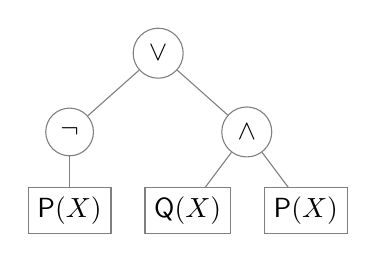
\begin{tikzpicture}
    \node[draw,circle,gray,text=black] (or) at (-0.375, 0) {$\lor$};
    \node[draw,circle,gray,text=black] (not) at (-1.5, -1) {$\neg$};
    \node[draw,circle,gray,text=black] (and) at (0.75, -1) {$\land$};
    \node[draw,gray,text=black] (P) at (-1.5, -2) {$\mathsf{P}(X)$};
    \node[draw,gray,text=black] (Q) at (0, -2) {$\mathsf{Q}(X)$};
    \node[draw,gray,text=black] (R) at (1.5, -2) {$\mathsf{P}(X)$};
    \draw[gray] (or) -- (not);
    \draw[gray] (or) -- (and);
    \draw[gray] (not) -- (P);
    \draw[gray] (and) -- (Q);
    \draw[gray] (and) -- (R);
  \end{tikzpicture}
  \caption{A tree representation of the formula from \cref{example:formula}}
  \label{fig:example_tree}
\end{figure}

\begin{example} \label{example:formula}
  Let $\maxNumNodes{} = 8$. Then
  \[
    \neg\mathsf{P}(X) \lor (\mathsf{Q}(X) \land \mathsf{P}(X))
  \]
  corresponds to the tree in \cref{fig:example_tree} and can be encoded as:
  \begin{alignat*}{8}
    \variable{structure} &= [0, &&0, &&0, &&1, &&2, &&2, &&6, &&7],\\
    \variable{values} &= [{\lor}, &&{\neg}, &&{\land}, \mathsf{P}(&&X), \mathsf{Q}(&&X), \mathsf{P}(&&X), &&\top, &&\top],\\
    \variable{numNodes} &= 6, && && && && && && &&\\
    \variable{numTrees} &= 3. && && && && && && &&
  \end{alignat*}
\end{example}

Here, $\top$ is the value we use for the remaining one-node trees. The
elements of the $\variable{values}$ array are \emph{nodes}.

\begin{definition} \label{def:node}
  A \emph{node} has a $\variable{name} \in \tokens{} \cup \predicates{}$ and
  $\arrayd{arguments}{\maxArity{}}{\variables{} \cup \constants{} \cup \{ \Box
    \}}$. The node's $\variable{arity}$ can then be
  defined analogously to \cref{def:arity}.
\end{definition}

Furthermore, we can use \cref{constr:arity} again to disable the extra
arguments.

\begin{example}
  Let $\maxArity{} = 2$, $X \in \variables{}$, and let $\mathsf{P}$ be a
  predicate with arity 1. Then the node representing atom $\mathsf{P}(X)$ has:
  \begin{align*}
    \variable{name} &= \mathsf{P},\\
    \variable{arguments} &= [X, \Box],\\
    \variable{arity} &= 1.
  \end{align*}
\end{example}

It remains to constrain the forest represented by the $\variable{structure}$
array together with its $\variable{values}$ to eliminate unnecessary symmetries
and adhere to our desired format. First, we can recognise that the order of the
elements in the $\variable{structure}$ array does not matter, i.e., the
structure is only defined by how the elements link to each other, so we can add
a constraint saying that:

\begin{constraint}
  \variable{structure} is sorted.
\end{constraint}

Next, since we already have a variable that counts the number of nodes in the
main tree, we can fix the structure and the values of the remaining trees to
some constant values:

\begin{constraint}
  For $i = 1, \dots, \maxNumNodes{} - 1$, if $i \ge \variable{numNodes}$, then
  \[
    \variable{structure}[i] = i, \quad \text{and} \quad
    \variable{values}[i].\variable{name} = \top,
  \]
  else $\variable{structure}[i] < i$.
\end{constraint}

The second part of this constraint states that every node in the main tree
except the zeroth node cannot be a root and must have its parent located to
the left of itself. Next, we classify all nodes into three classes: predicate
(or empty) nodes, negation nodes, and conjunction/disjunction nodes based on the
number of children (zero, one, and two, respectively).

\begin{constraint} \label{constraint:node_types}
  For $i = 0, \dots, \maxNumNodes{} - 1$, let $C_i$ be the number of times $i$
  appears in the \variable{struture} array with index greater than $i$. Then
  \begin{align*}
    C_i = 0 &\iff \variable{values}[i].\variable{name} \in \predicates{} \cup \{ \top \},\\
    C_i = 1 &\iff \variable{values}[i].\variable{name} = \neg,\\
    C_i > 1 &\iff \variable{values}[i].\variable{name} \in \{ \land, \lor \}.
  \end{align*}
\end{constraint}

The value $\top$ serves a twofold purpose: it is used as the fixed value for
nodes outside the main tree, and, when located at the zeroth node, it can
represent a clause with no body. Thus, we can say that only root nodes can have
$\top$ as the value:

\begin{constraint}
  For $i = 0, \dots, \maxNumNodes{} - 1$,
  \[
    \variable{structure}[i] \ne i \implies
    \variable{values}[i].\variable{name} \ne \top.
  \]
\end{constraint}

Finally, we add a way to disable a clause by setting its head predicate to
$\Box$:

\begin{constraint}
  For $i = 0, \dots, \maxNumClauses{} - 1$, if
  $\variable{heads}[i].\variable{predicate} = \Box$, then
  \[
    \variable{bodies}[i].\variable{numNodes} = 1,
  \]
  and
  \[
    \variable{bodies}[i].\variable{values}[0].\variable{name} =
    \top.
  \]
\end{constraint}

\section{VARIABLE SYMMETRIES} \label{sec:variable_symmetry}

Given any clause, we can permute the variables in it without changing the
meaning of the clause or the entire program. Thus, we want to fix the order of
variables to eliminate unnecessary symmetries. Informally, we can say that
variable $X$ goes before variable $Y$ if its first occurrence in either the head
or the body of the clause is before the first occurrence of $Y$. Note that the
constrains described in this section only make sense if $|\variables| > 1$. Also
note that all definitions and constraints here are on a per-clause basis.

\begin{definition}
  Let $N = \maxArity{} \times (\maxNumNodes{} + 1)$. Let
  $\variable{terms}[N] \in \constants{} \cup \variables{} \cup \{ \Box
  \}$ be a flattened array of all arguments in a particular clause.

  Then we can use the $\variable{setsIntsChanneling}$ constraint
  to define $\variable{occ}[|\constants{}| + |\variables{}| + 1]$ as an
  array of subsets of $\{ 0, \dots, N-1 \}$ such that for all $i = 0, \dots, N
  - 1$, and $t \in \constants{} \cup \variables{} \cup \{ \Box \}$,
  \[
    i \in \variable{occ}[t] \quad \iff \quad
    \variable{terms}[i] = t
  \]
\end{definition}

We introduce an array that, for each variable, holds the position of its first
occurrence.
\begin{definition}
  Let $\arrayd{intros}{|\variables{}|}{\{ 0, \dots, N \}}$ be such that
  for $v \in \variables{}$,
  \[
    \variable{intros}[v] = \begin{cases}
      1 + \min \variable{occ}[v] & \text{if }
      \variable{occ}[v] \ne \emptyset\\
      0 & \text{otherwise.}
    \end{cases}
  \]
\end{definition}
Here, a value of zero means that the variable does not occur in the clause. We
want to use specifically zero for this so that we could use
\cref{constraint:diffbutzero} later. Because of this choice, the definition of
$\variable{intros}$ shifts all indices by one.

\begin{constraint}
  $\variable{intros}$ are sorted.
\end{constraint}

\begin{example} \label{example:sibling}
  Let $\constants{} = \emptyset$, $\variables{} = \{ X, Y, Z \}$, $\maxArity{} =
  2$, $\maxNumNodes{} = 3$, and consider the clause
  \[
    \mathsf{sibling}(X, Y) \gets \mathsf{parent}(X, Z) \land
    \mathsf{parent}(Y, Z).
  \]
  Then $\variable{terms} = [X, Y, \Box, \Box, X, Z, Y, Z]$ (the boxes represent
  the conjunction node), $\variable{occ} = [\{ 0, 4 \}, \{ 1, 6 \},
  \{ 5, 7 \}, \{ 2, 3 \}]$, and $\variable{intros} = [0, 1, 5]$.
\end{example}

\subsection{REDUNDANT CONSTRAINTS}

We add a number of redundant constraints to make search more efficient.

\begin{constraint}
  For $u \ne v \in \constants{} \cup \variables{} \cup \{ \Box \}$,
  \[
    \variable{occ}[u] \cap \variable{occ}[v] = \emptyset.
  \]
\end{constraint}

\begin{constraint} \label{constraint:diffbutzero}
  $\variable{allDifferentExcept0}(\variable{intros})$.
\end{constraint}

\begin{constraint}
  For $v \in \variables{}$,
  \[
    \variable{intros}[v] \ne 0 \quad \iff \quad
    \variable{intros}[v] - 1 \in \variable{occ}[v].
  \]
\end{constraint}

\begin{definition}
  We define an auxiliary set variable
  \[
    \variable{potentialIntros} \subseteq \{ 0, \dots, N \}
  \]
  to act as a set of possible values that $\variable{intros}$ can take,
  i.e., for $v \in \variables{}$, $\variable{intros}[v] \in
  \variable{potentialIntros}$.
\end{definition}

\begin{constraint} \label{constraint:potentialIntroductions}
  For $i = 0, \dots, \maxNumNodes{} - 1$, let
  \[
    S = \{ \maxArity{} \times (i + 1) + j + 1 \mid j = 0, \dots, \maxArity{} - 1.
    \}
  \]
  If $\variable{values}[i].\variable{name} \not\in \predicates{}$, then
  \[
    \variable{potentialIntros} \cap S = \emptyset.
  \]
\end{constraint}
In simpler terms, \cref{constraint:potentialIntroductions} says that if a node
in the tree representation of a clause represents something other than a
predicate, then a variable cannot be introduced as one of its `arguments'.

\section{COUNTING PROGRAMS}

In order to demonstrate the correctness of the model and explain it in more
detail, in this section we are going to derive combinatorial expressions for
counting the number of programs with up to $\maxNumClauses{}$ clauses and up to
$\maxNumNodes{}$ nodes per clause, and arbitrary $\predicates{}$,
$\arities{}$, $\variables{}$, and $\constants{}$. To simplify the task, we only
consider clauses without probabilities and disable (negative) cycle elimination.
It was experimentally confirmed that the model agrees with the combinatorial
formula from this section in 985 different scenarios. The \emph{total arity} of
a body of a clause is the sum total of arities of all predicates in the body.

We will first consider clauses with gaps, i.e., without taking variables and
constants into account. Let $T(n, a)$ denote the number of possible clause
bodies with $n$ nodes and total arity $a$. Then $T(1, a)$ is the number of
predicates in $\predicates{}$ with arity $a$, and the following recursive
definition can be applied for $n > 1$:
\begin{align*}
  T(n, a) = T(n-1, a) + 2&\sum_{\substack{c_1 + \dots + c_k = n - 1,\\
      2 \le k \le \frac{a}{\min \arities{}},\\
  c_i \ge 1 \text{ for all } i}}\\
  &\sum_{\substack{d_1 + \dots + d_k = a,\\
  d_i \ge \min \arities{} \text{ for all } i}} \prod_{i=1}^k T(c_i, d_i).
\end{align*}
The first term here represents negation, i.e., negating an expression consumes
one node but otherwise leaves the task unchanged. If the first operation is not
negation, then it must be either conjunction or disjunction (hence the
coefficient `2'). In the first sum, $k$ represents the number of children of the
root node, and each $c_i$ is the number of nodes dedicated to child $i$. Thus,
the first sum iterates over all possible ways to partition the remaining $n-1$
nodes. Similarly, the second sum considers every possible way to partition the
total arity $a$ across the $k$ children nodes.

We can then count the number of possible clause bodies with total arity $a$ (and
any number of nodes) as
\[
  C(a) = \begin{cases}
    1 & \text{if } a = 0\\
    \sum_{n=1}^{\maxNumNodes{}} T(n, a) & \text{otherwise.}
  \end{cases}
\]
Here, the empty clause is considered separately.

The number of ways to select $n$ terms is
\begin{align*}
  P(n) = |\constants{}|^n + &\sum_{\substack{1 \le k \le |\variables{}|, \\ 0 =
      s_0 < s_1 < \dots < s_k < s_{k+1} = n+1}}\\
  &\prod_{i=0}^k (|\constants{}| + i)^{s_{i+1} - s_i - 1}.
\end{align*}
The first term is the number of ways select $n$ constants. The parameter $k$ is
the number of variables used in the clause, and $s_1, \dots, s_k$ mark the first
occurrence of each variable. For each gap between any two introductions (or
before the first introduction, or after the last introduction), we have
$s_{i+1}-s_i-1$ spaces to be filled with any of the $|\constants{}|$ constants
or any of the $i$ already-introduced variables.

Let us order the elements of $\predicates{}$, and let $a_i$ be the arity of the
$i$-th predicate. The number of programs is then:
\[
  \sum_{\substack{ \sum_{i=1}^{|\predicates{}|} h_i = n,\\
      |\predicates{}| \le n \le \maxNumClauses,\\
      h_i \ge 1 \text{ for all } i}} \prod_{i=1}^{|\predicates{}|}
  \multiset{\sum_{a=0}^{\maxArity{} \times \maxNumNodes{}} C(a) P(a+a_i)}{h_i},
\]
where
\[
  \multiset{n}{k} = \binom{n+k-1}{k}
\]
counts the number of ways to select $k$ out of $n$ items with repetition (and
without ordering). Here, we sum over all possible ways to distribute
$|\predicates{}| \le n \le \maxNumClauses{}$ clauses among $|\predicates{}|$
predicates so that each predicate gets at least one clause. For each predicate,
we can then count the number of ways to select its clauses out of all possible
clauses. The number of possible clauses can be computed by considering each
possible arity $a$, and multiplying the number of `unfinished' clauses $C(a)$ by
the number of ways to select the required $a+a_i$ terms in the body and the head
of the clause.

\section{PREDICATE INDEPENDENCE} \label{sec:independence}

In this section, we define a notion of predicate independence as a way to
constrain the probability distributions defined by the generated programs. We
also describe efficient algorithms for propagation and entailment checking.

\begin{definition}
  Let $\mathscr{P}$ be a probabilistic logic program. Its \emph{predicate
    dependency graph} is a directed graph $G_{\mathscr{P}} = (V, E)$ with the
  set of nodes $V$ consisting of all predicates in $\mathscr{P}$. For any two
  different predicates $\mathsf{P}$ and $\mathsf{Q}$, we add an edge from
  $\mathsf{P}$ to $\mathsf{Q}$ if there is a clause in $\mathscr{P}$ with
  $\mathsf{Q}$ as the head and $\mathsf{P}$ mentioned in the body. We say that
  the edge is \emph{negative} if there exists a clause with $\mathsf{Q}$ as the
  head and at least one instance of $\mathsf{P}$ at the body such that the path
  from the root to the $\mathsf{P}$ node in the tree representation of the
  clause passes through at least one negation node. Otherwise it is
  \emph{positive}. We say that $\mathscr{P}$ (or $G_{\mathscr{P}}$) has a
  \emph{negative cycle} if $G_{\mathscr{P}}$ has a cycle with at least one
  negative edge.
\end{definition}

\begin{definition}
  Let $\mathsf{P}$ be a predicate in a program $\mathscr{P}$. The set of
  \emph{dependencies} of $\mathsf{P}$ is the smallest set $D_{\mathsf{P}}$ such
  that:
  \begin{itemize}
  \item $\mathsf{P} \in D_{\mathsf{P}}$,
  \item for every $\mathsf{Q} \in D_{\mathsf{P}}$, all direct predecessors of
    $\mathsf{Q}$ in $G_{\mathscr{P}}$ are in $D_{\mathsf{P}}$.
  \end{itemize}
\end{definition}

\begin{definition}
  Two predicates $\mathsf{P}$ and $\mathsf{Q}$ are \emph{independent} if
  $D_{\mathsf{P}} \cap D_{\mathsf{Q}} = \emptyset$.
\end{definition}

\begin{figure}
  \centering
  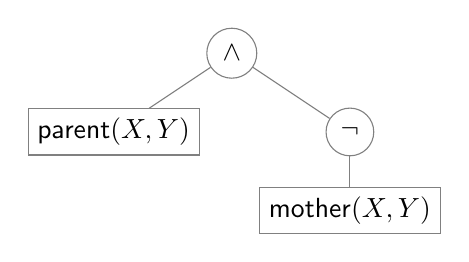
\begin{tikzpicture}
    \node[draw,circle,gray,text=black] (and) at (0, 0) {$\land$};
    \node[draw,circle,gray,text=black] (not) at (1.5, -1) {$\neg$};
    \node[draw,gray,text=black] (parent) at (-1.5, -1) {$\mathsf{parent}(X, Y)$};
    \node[draw,gray,text=black] (mother) at (1.5, -2) {$\mathsf{mother}(X, Y)$};
    \draw[gray] (and) -- (parent);
    \draw[gray] (and) -- (not);
    \draw[gray] (not) -- (mother);
  \end{tikzpicture}
  \caption{A tree representation of the body of \cref{eq:example_clause}}
  \label{fig:example_tree2}
\end{figure}
\begin{figure}
  \centering
  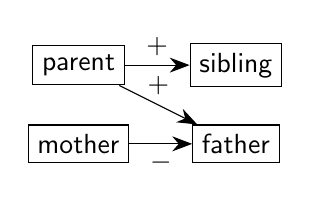
\begin{tikzpicture}
    \node[draw] (parent) at (0, 0.5) {$\mathsf{parent}$};
    \node[draw] (mother) at (0, -0.5) {$\mathsf{mother}$};
    \node[draw] (sibling) at (2, 0.5) {$\mathsf{sibling}$};
    \node[draw] (father) at (2, -0.5) {$\mathsf{father}$};
    \draw[-{Stealth[scale=1.5]}] (parent) edge node[above] {$+$} (sibling);
    \draw[-{Stealth[scale=1.5]}] (parent) edge node[above] {$+$} (father);
    \draw[-{Stealth[scale=1.5]}] (mother) edge node[below] {$-$} (father);
  \end{tikzpicture}
  \caption{The predicate dependency graph of the program in \cref{ex:program}.
    Positive edges are labelled with `$+$', and negative edges with `$-$'.}
  \label{fig:predicate_dependencies}
\end{figure}

\begin{example} \label{ex:program}
  Consider the following (fragment of a) program:
  \begin{align}
    \mathsf{sibling}(X, Y) &\gets \mathsf{parent}(X, Z) \land \mathsf{parent}(Y, Z), \nonumber \\
    \mathsf{father}(X, Y) &\gets \mathsf{parent}(X, Y) \land \neg\mathsf{mother}(X, Y). \label[clause]{eq:example_clause}
  \end{align}
  Its predicate dependency graph is in \cref{fig:predicate_dependencies}.
  Because of the negation in \cref{eq:example_clause} (as seen in
  \cref{fig:example_tree2}), the edge from $\mathsf{mother}$ to
  $\mathsf{father}$ is negative, while the other two edges are positive.

  We can now list the dependencies of each predicate:
  \begin{alignat*}{3}
    D_{\mathsf{parent}} &= \{ \mathsf{parent} \}, && D_{\mathsf{sibling}}
    &&= \{\mathsf{sibling}, \mathsf{parent} \},\\
    D_{\mathsf{mother}} &= \{ \mathsf{mother} \}, && D_{\mathsf{father}}
    &&= \{ \mathsf{father}, \mathsf{mother}, \mathsf{parent} \}.
  \end{alignat*}
  Hence, we have two pairs of independent predicates, i.e., $\mathsf{mother}$ is
  independent from $\mathsf{parent}$ and $\mathsf{sibling}$.
\end{example}

We can now add a constraint to define an adjacency matrix for the predicate
dependency graph but without positivity/negativity.
\begin{definition} \label{def:adjacency_matrix}
  An $|\predicates{}| \times |\predicates{}|$ adjacency matrix $\mathbf{A}$ with
  $\{ 0, 1 \}$ as its domain is defined by stating that $\mathbf{A}[i][j] = 0$
  if and only if, for all $k \in \{ 0, \dots, \maxNumClauses{} - 1 \}$, either
  \[
    \variable{heads}[k].\variable{predicate} \ne j
  \]
  or
  \[
    i \not\in \{a.\variable{name} \mid a \in
    \variable{bodies}[k].\variable{values} \}.
  \]
\end{definition}

Given an undetermined model, we can classify all dependencies of a predicate
$\mathsf{P}$ into three categories based on how many of the edges on the path
from the dependency to $\mathsf{P}$ are undetermined. In the case of zero, we
call the dependency \emph{determined}. In the case of one, we call it
\emph{almost determined}. Otherwise, it is \emph{undetermined}. In the context
of propagation and entailment algorithms, we define a \emph{dependency} as the
sum type:
\begin{grammar}
  <dependency> ::= $\Determined(p)$ | $\Undetermined(p)$ | $\AlmostDetermined(p,
  s, t)$
\end{grammar}
where each alternative represents a determined, undetermined, and almost
determined dependency, respectively. Here, $p \in \predicates{}$ is the name of
the predicate which is the dependency of $\mathsf{P}$, and---in the case of
$\AlmostDetermined$---$(s, t) \in \predicates{}^2$ is the one undetermined edge
in $\mathbf{A}$ that prevents the dependency from being determined. For a
dependency $d$---regardless of its exact type---we will refer to its predicate
$p$ as $d.\mathsf{predicate}$. In describing the algorithms, we will use an
underscore to replace any of $p$, $s$, $t$ in situations where the name is
unimportant.

\begin{algorithm}
  \SetKwFunction{getDependencies}{deps}
  \SetKwFunction{isDetermined}{isDetermined}
  \SetKwData{predicate}{predicate}
  \KwData{predicates $p_1$, $p_2$}
  \nosemic $D \gets \{ (d_1, d_2) \in \getDependencies{$p_1$, 1} \times \getDependencies{$p_2$, 1}$\;
  \hspace{27pt}\dosemic $\mid d_1.\predicate = d_2.\predicate \}$\;
  \lIf{$D = \emptyset$}{\Return{\textsc{true}}}
  \lIf{$\exists (\Determined \_, \Determined \_) \in D$}{\Return{\textsc{false}}}
  \Return{\textsc{undefined}}\;
  \caption{Entailment for independence}
  \label{alg:independence_entailment}
\end{algorithm}

Each entailment algorithm returns one out of three different values:
\textsc{true} if the constraint is guaranteed to hold, \textsc{false} if the
constraint is violated, and \textsc{undefined} if whether the constraint will be
satisfied or not depends on the future decisions made by the solver.
\cref{alg:independence_entailment} outlines a simple entailment algorithm for
the independence of two predicates $p_1$ and $p_2$. First, we separately
calculate all dependencies of $p_1$ and $p_2$, and look at the set $D$ of
dependencies that $p_1$ and $p_2$ have in common. If there are none, then the
predicates are clearly independent. If they have a dependency in common that is
already fully determined ($\Determined$) for both predicates, then they cannot be
independent. Otherwise, we return \textsc{undefined}.

\begin{algorithm}
  \LinesNumbered
  \SetKwFunction{getDependencies}{deps}
  \SetKwFunction{fail}{fail}
  \SetKwFunction{removeValue}{removeValue}
  \SetKwData{predicate}{predicate}
  \SetKwData{source}{source}
  \SetKwData{target}{target}
  \KwData{predicates $p_1$, $p_2$; adjacency matrix $\mathbf{A}$}
  \For{$(d_1, d_2) \in \getDependencies{$p_1$, 0} \times \getDependencies{$p_2$,
      0}$ such that $d_1.\predicate = d_2.\predicate$}{
    \lIf{$d_1$ {\bf is} $\Determined(\_)$ {\bf and} $d_2$ {\bf is}
      $\Determined(\_)$}{\fail{}} \label{line:fail}
    \If{$d_1$ {\bf is} $\Determined(\_)$ {\bf and} $d_2$ {\bf is}
      $\AlmostDetermined(\_, s, t)$ {\bf or} \hspace{50pt} $d_2$ {\bf is}
      $\Determined(\_)$ {\bf and} $d_1$ {\bf is} $\AlmostDetermined(\_, s,
      t)$ \label{line:propagation_condition}}{
      $\mathbf{A}[s][t]$.\removeValue{$1$}\; \label{line:propagation_result}
    }
  }
  \caption{Propagation for independence}
  \label{alg:independence_propagation}
\end{algorithm}

Propagation algorithms have two goals: causing a contradiction (failing) in
situations where the corresponding entailment algorithm would return
\textsc{false}, and eliminating values from domains of variables that are
guaranteed to cause a contradiction. \cref{alg:independence_propagation} does
the former on \cref{line:fail}. Furthermore, for any dependency shared between
predicates $p_1$ and $p_2$, if it is determined ($\Determined$) for one
predicate and almost determined ($\AlmostDetermined$) for another, then the edge
that prevents the $\AlmostDetermined$ from becoming a $\Determined$ cannot
exist--\cref{line:propagation_condition,line:propagation_result} take care of
that.

\begin{algorithm}
  \SetKwData{edgeExists}{edge}
  \SetKwData{predicate}{predicate}
  \SetKwData{source}{source}
  \SetKwData{target}{target}
  \SetKwData{all}{allDependencies}
  \SetKwFunction{getDependencies}{deps}
  \SetKwProg{Fn}{Function}{:}{}
  \KwData{adjacency matrix $\mathbf{A}$}
  \Fn{\getDependencies{$p$, \all}} {
    $D \gets \{ \Determined(p) \}$\;
    \While{\logical{true}}{
      $D' \gets \emptyset$\;
      \For{$d \in D$ {\bf and} $q \in \predicates{}$}{
        $\edgeExists \gets \mathbf{A}[q][d.\predicate] = \{ 1 \}$\;
        \uIf{$\edgeExists$ {\bf and} $d$ {\bf is} $\Determined(\_)$}{
          $D' \gets D' \cup \{ \Determined(q) \}$
        }
        \uElseIf{$\edgeExists$ {\bf and} $d$ {\bf is} $\AlmostDetermined(\_, s,
          t)$}{
          $D' \gets D' \cup \{ \AlmostDetermined(q, s, t) \}$\;
        }
        \uElseIf{$|\mathbf{A}[q][d.\predicate]| > 1$ {\bf and} $d$~{\bf is}~$\Determined(r)$}{
          $D' \gets D' \cup \{ \AlmostDetermined(q, q, r) \}$\;
        }
        \ElseIf{$|\mathbf{A}[q][d.\predicate]| > 1$ {\bf and} \all}{
          $D' \gets D' \cup \{ \Undetermined(q) \}$\;
        }
      }
      \lIf{$D' = D$}{\Return{$D$}}
      $D \gets D'$\;
    }
  }
  \caption{Dependencies of a predicate}
  \label{alg:dependencies}
\end{algorithm}

The function $\getDependencies$ in \cref{alg:dependencies} calculates $D_p$ for
any predicate $p$. It has two versions: $\getDependencies(p, 1)$ returns all
dependencies, while $\getDependencies(p, 0)$ returns only determined and
almost-determined dependencies. It starts by establishing the predicate $p$
itself as a dependence and continues to add dependencies of dependencies until
the set $D$ stabilises. For each dependency $d \in D$, we look at the in-links
of $d$ in the predicate dependency graph. If the edge from some predicate $q$ to
$d.\mathsf{predicate}$ is fully determined and $d$ is determined, then $q$ is
another determined dependency of $p$. If the edge is determined but $d$ is
almost determined, then $q$ is an almost-determined dependency. The same outcome
applies if $d$ is fully determined but the edge is undetermined. Finally, if we
are interested in collecting all dependencies regardless of their status, then
$q$ is a dependency of $p$ as long as the edge from $q$ to
$d.\mathsf{predicate}$ is possible. Note that if there are multiple paths in the
dependency graph from $q$ to $p$, \cref{alg:dependencies} could include $q$ once
for each possible type ($\Determined$, $\Undetermined$, and
$\AlmostDetermined$), but
\cref{alg:independence_propagation,alg:independence_entailment} would still work
as intended.

\begin{figure}
  \centering
  \[
    \begin{blockarray}{ccccc}
      \begin{block}{c(cccc)}
        \mathsf{father} & 0 & 0 & 0 & 0 \\
        \mathsf{mother} & 1 & 0 & 0 & 0 \\
        \mathsf{parent} & 1 & \fbox{\{ 0, 1 \}} & \{ 0, 1 \} & \{ 0, 1 \} \\
        \mathsf{sibling} & 0 & 0 & 0 & 0 \\
      \end{block}
    \end{blockarray}
  \]
  \caption{The adjacency matrix defined using \cref{def:adjacency_matrix} for
    \cref{example:independence}}
  \label{fig:dependencies_matrix}
\end{figure}

\begin{figure}
  \centering
  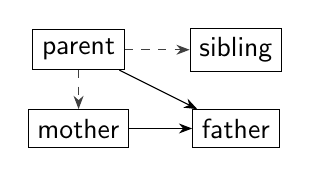
\begin{tikzpicture}
    \node[draw] (parent) at (0, 0.5) {$\mathsf{parent}$};
    \node[draw] (mother) at (0, -0.5) {$\mathsf{mother}$};
    \node[draw] (sibling) at (2, 0.5) {$\mathsf{sibling}$};
    \node[draw] (father) at (2, -0.5) {$\mathsf{father}$};
    \draw[-{Stealth}] (parent) edge (father);
    \draw[-{Stealth}] (mother) edge (father);
    \draw[-{Stealth},dashed,darkgray] (parent) edge (sibling);
    \draw[-{Stealth},dashed,darkgray] (parent) edge (mother);
  \end{tikzpicture}
  \caption{The predicate dependency graph that corresponds to
    \cref{fig:dependencies_matrix}. Dashed edges are undetermined---they may
    or may not exist.}
  \label{fig:dependencies2}
\end{figure}

\begin{example} \label{example:independence}
  Consider this partially determined (fragment of a) program:
  \begin{align*}
    \Box(X, Y) &\gets \mathsf{parent}(X, Z) \land \mathsf{parent}(Y, Z),\\
    \mathsf{father}(X, Y) &\gets \mathsf{parent}(X, Y) \land \neg\mathsf{mother}(X, Y)
  \end{align*}
  where $\Box$ indicates an unknown predicate with domain
  \[
    D = \{ \mathsf{father}, \mathsf{mother}, \mathsf{parent}, \mathsf{sibling}
    \}.
  \]
  The predicate dependency graph (without positivity/negativity) defined by
  \cref{def:adjacency_matrix} is represented in
  \cref{fig:dependencies_matrix,fig:dependencies2}.

  Suppose we have a constraint that $\mathsf{mother}$ and $\mathsf{parent}$ must
  be independent. The lists of potential dependencies for both predicates are:
  \begin{align*}
    D_{\mathsf{mother}} &= \{ \Determined(\mathsf{mother}), \AlmostDetermined(\mathsf{parent}, \mathsf{parent}, \mathsf{mother}) \}, \\
    D_{\mathsf{parent}} &= \{ \Determined(\mathsf{parent}) \}.
  \end{align*}
  An entailment check at this stage would produce \textsc{undefined}, but
  propagation replaces the boxed value in \cref{fig:dependencies_matrix} with
  zero, eliminating the potential edge from $\mathsf{parent}$ to
  $\mathsf{mother}$. This also eliminates $\mathsf{mother}$ from $D$, and,
  although some undetermined variables remain, this is enough to make
  \cref{alg:independence_entailment} return \textsc{true}.
\end{example}

\section{NEGATIVE CYCLES} \label{sec:cycles}
% TODO: My paper has two slightly different graphs with the same name.
% TODO: NB: the set of decision variables for this constraint must exclude all
% arguments.
% TODO: maybe move some of the definition 10 here.

Having no negative cycles in the predicate dependency graph is a requirement for
probabilistic logic programming language ProbLog \citep{kimmig2009trading},
although it has been shown how the requirement can be alleviated by introducing
negative probabilities \citep{DBLP:journals/ijar/BuchmanP17}. Ideally, we would
like to design a constraint for that similar to the constraint for independence
in the previous section. However, the difficulty with creating a propagation
algorithm for negative cycles is that there seems to be no good way to extend
\cref{def:adjacency_matrix} so that the adjacency matrix captures
positivity/negativity. Thus, we settle for an entailment algorithm with no
propagation.

\begin{algorithm}
  \KwData{a program $\mathscr{P}$}
  \SetKwFunction{hasNegativeCycles}{hasNegativeCycles}
  Let $\mathscr{R} \subseteq \mathscr{P}$ be the largest subprogram of
  $\mathscr{P}$ with its $\variable{structure}$ and predicates in both body
  and head fully determined\footnotemark\;
  \If{\hasNegativeCycles($G_{\mathscr{R}}$)}{
    \Return{\textsc{false}}\;
  }
  \lIf{$\mathscr{R} = \mathscr{P}$}{\Return{\textsc{true}}}
  \Return{\textsc{undefined}}\;
  \caption{Entailment for negative cycles}
  \label{alg:negative_cycles}
\end{algorithm}
\footnotetext{The arguments (whether variables or constants) are irrelevant to
  our definition of independence.}

The algorithm takes all clauses whose structure and predicates have been fully
determined and uses them to construct a full dependency graph. In our
implementation, \texttt{hasNegativeCycles} function is just a simple extension
of the backtracking cycle detection algorithm that `travels' around the graph
following edges and checking if each vertex has already been visited or not.
Alternatively, one could assign weights to the edges (e.g., $1$ for positive
and $-\infty$ for negative edges), thus reducing our negative cycle detection
problem to what is typically known as the negative cycle detection problem in
the literature, and use an algorithm such as Bellman-Ford
\citep{shimbel1954structure}.

If the algorithm finds a negative cycle in this fully-determined part of the
program, then it is unavoidable and we must return \textsc{false}. If there was
no negative cycle and the entire program is determined-enough to contribute to
the graph, then there cannot be any negative cycles. In all other cases, it
is too early to tell.

\section{EMPIRICAL PERFORMANCE}

\begin{figure}
  \centering
  % Created by tikzDevice version 0.12.3 on 2020-01-22 11:34:15
% !TEX encoding = UTF-8 Unicode
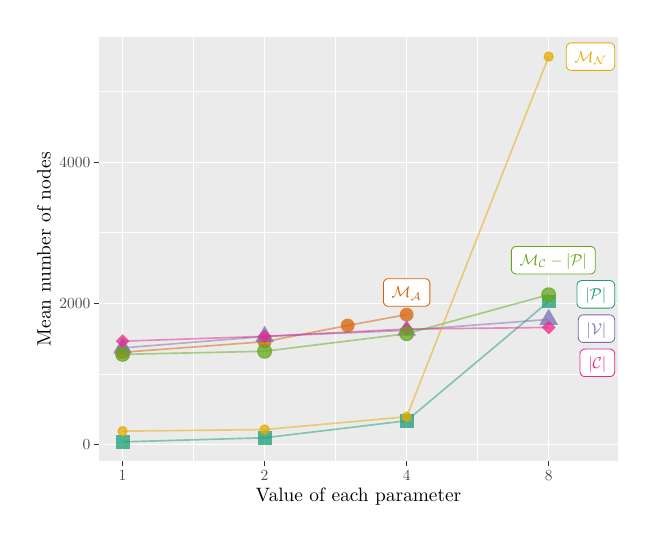
\begin{tikzpicture}[x=1pt,y=1pt]
\definecolor{fillColor}{RGB}{255,255,255}
\path[use as bounding box,fill=fillColor,fill opacity=0.00] (0,0) rectangle (216.81,176.16);
\begin{scope}
\path[clip] (  0.00,  0.00) rectangle (216.81,176.16);
\definecolor{drawColor}{RGB}{255,255,255}
\definecolor{fillColor}{RGB}{255,255,255}

\path[draw=drawColor,line width= 0.4pt,line join=round,line cap=round,fill=fillColor] (  0.00,  0.00) rectangle (216.81,176.16);
\end{scope}
\begin{scope}
\path[clip] ( 25.78, 19.53) rectangle (213.31,172.66);
\definecolor{fillColor}{gray}{0.92}

\path[fill=fillColor] ( 25.78, 19.53) rectangle (213.31,172.66);
\definecolor{drawColor}{RGB}{255,255,255}

\path[draw=drawColor,line width= 0.2pt,line join=round] ( 25.78, 51.08) --
	(213.31, 51.08);

\path[draw=drawColor,line width= 0.2pt,line join=round] ( 25.78,102.07) --
	(213.31,102.07);

\path[draw=drawColor,line width= 0.2pt,line join=round] ( 25.78,153.07) --
	(213.31,153.07);

\path[draw=drawColor,line width= 0.2pt,line join=round] ( 59.96, 19.53) --
	( 59.96,172.66);

\path[draw=drawColor,line width= 0.2pt,line join=round] (111.28, 19.53) --
	(111.28,172.66);

\path[draw=drawColor,line width= 0.2pt,line join=round] (162.60, 19.53) --
	(162.60,172.66);

\path[draw=drawColor,line width= 0.4pt,line join=round] ( 25.78, 25.58) --
	(213.31, 25.58);

\path[draw=drawColor,line width= 0.4pt,line join=round] ( 25.78, 76.58) --
	(213.31, 76.58);

\path[draw=drawColor,line width= 0.4pt,line join=round] ( 25.78,127.57) --
	(213.31,127.57);

\path[draw=drawColor,line width= 0.4pt,line join=round] ( 34.30, 19.53) --
	( 34.30,172.66);

\path[draw=drawColor,line width= 0.4pt,line join=round] ( 85.62, 19.53) --
	( 85.62,172.66);

\path[draw=drawColor,line width= 0.4pt,line join=round] (136.94, 19.53) --
	(136.94,172.66);

\path[draw=drawColor,line width= 0.4pt,line join=round] (188.26, 19.53) --
	(188.26,172.66);
\definecolor{drawColor}{RGB}{27,158,119}

\path[draw=drawColor,draw opacity=0.50,line width= 0.6pt,line join=round] ( 34.30, 26.49) --
	( 85.62, 27.97) --
	(136.94, 34.12) --
	(188.26, 77.20);
\definecolor{drawColor}{RGB}{217,95,2}

\path[draw=drawColor,draw opacity=0.50,line width= 0.6pt,line join=round] ( 34.30, 58.87) --
	( 85.62, 62.68) --
	(115.64, 68.55) --
	(136.94, 72.47);
\definecolor{drawColor}{RGB}{117,112,179}

\path[draw=drawColor,draw opacity=0.50,line width= 0.6pt,line join=round] ( 34.30, 60.44) --
	( 85.62, 64.58) --
	(136.94, 66.81) --
	(188.26, 70.73);
\definecolor{drawColor}{RGB}{231,41,138}

\path[draw=drawColor,draw opacity=0.50,line width= 0.6pt,line join=round] ( 34.30, 62.87) --
	( 85.62, 64.62) --
	(136.94, 67.25) --
	(188.26, 67.83);
\definecolor{drawColor}{RGB}{102,166,30}

\path[draw=drawColor,draw opacity=0.50,line width= 0.6pt,line join=round] ( 34.30, 58.10) --
	( 85.62, 59.23) --
	(136.94, 65.57) --
	(188.26, 79.66);
\definecolor{drawColor}{RGB}{230,171,2}

\path[draw=drawColor,draw opacity=0.50,line width= 0.6pt,line join=round] ( 34.30, 30.36) --
	( 85.62, 30.94) --
	(136.94, 35.55) --
	(188.26,165.70);
\definecolor{fillColor}{RGB}{27,158,119}

\path[fill=fillColor,fill opacity=0.75] ( 31.81, 23.99) --
	( 36.80, 23.99) --
	( 36.80, 28.99) --
	( 31.81, 28.99) --
	cycle;

\path[fill=fillColor,fill opacity=0.75] ( 83.13, 25.47) --
	( 88.12, 25.47) --
	( 88.12, 30.46) --
	( 83.13, 30.46) --
	cycle;

\path[fill=fillColor,fill opacity=0.75] (134.45, 31.63) --
	(139.44, 31.63) --
	(139.44, 36.62) --
	(134.45, 36.62) --
	cycle;

\path[fill=fillColor,fill opacity=0.75] (185.77, 74.70) --
	(190.76, 74.70) --
	(190.76, 79.69) --
	(185.77, 79.69) --
	cycle;
\definecolor{fillColor}{RGB}{217,95,2}

\path[fill=fillColor,fill opacity=0.75] ( 34.30, 58.87) circle (  2.50);

\path[fill=fillColor,fill opacity=0.75] ( 85.62, 62.68) circle (  2.50);

\path[fill=fillColor,fill opacity=0.75] (115.64, 68.55) circle (  2.50);

\path[fill=fillColor,fill opacity=0.75] (136.94, 72.47) circle (  2.50);
\definecolor{fillColor}{RGB}{117,112,179}

\path[fill=fillColor,fill opacity=0.75] ( 34.30, 64.32) --
	( 37.67, 58.50) --
	( 30.94, 58.50) --
	cycle;

\path[fill=fillColor,fill opacity=0.75] ( 85.62, 68.46) --
	( 88.99, 62.64) --
	( 82.26, 62.64) --
	cycle;

\path[fill=fillColor,fill opacity=0.75] (136.94, 70.70) --
	(140.31, 64.87) --
	(133.58, 64.87) --
	cycle;

\path[fill=fillColor,fill opacity=0.75] (188.26, 74.62) --
	(191.63, 68.79) --
	(184.90, 68.79) --
	cycle;
\definecolor{fillColor}{RGB}{231,41,138}

\path[fill=fillColor,fill opacity=0.75] ( 31.81, 62.87) --
	( 34.30, 65.37) --
	( 36.80, 62.87) --
	( 34.30, 60.37) --
	cycle;

\path[fill=fillColor,fill opacity=0.75] ( 83.13, 64.62) --
	( 85.62, 67.11) --
	( 88.12, 64.62) --
	( 85.62, 62.12) --
	cycle;

\path[fill=fillColor,fill opacity=0.75] (134.45, 67.25) --
	(136.94, 69.74) --
	(139.44, 67.25) --
	(136.94, 64.75) --
	cycle;

\path[fill=fillColor,fill opacity=0.75] (185.77, 67.83) --
	(188.26, 70.32) --
	(190.76, 67.83) --
	(188.26, 65.33) --
	cycle;
\definecolor{drawColor}{RGB}{102,166,30}
\definecolor{fillColor}{RGB}{102,166,30}

\path[draw=drawColor,draw opacity=0.75,line width= 0.4pt,line join=round,line cap=round,fill=fillColor,fill opacity=0.75] ( 34.30, 58.10) circle (  2.50);

\path[draw=drawColor,draw opacity=0.75,line width= 0.4pt,line join=round,line cap=round,fill=fillColor,fill opacity=0.75] ( 85.62, 59.23) circle (  2.50);

\path[draw=drawColor,draw opacity=0.75,line width= 0.4pt,line join=round,line cap=round,fill=fillColor,fill opacity=0.75] (136.94, 65.57) circle (  2.50);

\path[draw=drawColor,draw opacity=0.75,line width= 0.4pt,line join=round,line cap=round,fill=fillColor,fill opacity=0.75] (188.26, 79.66) circle (  2.50);
\definecolor{drawColor}{RGB}{230,171,2}
\definecolor{fillColor}{RGB}{230,171,2}

\path[draw=drawColor,draw opacity=0.75,line width= 0.4pt,line join=round,line cap=round,fill=fillColor,fill opacity=0.75] ( 34.30, 30.36) circle (  1.67);

\path[draw=drawColor,draw opacity=0.75,line width= 0.4pt,line join=round,line cap=round,fill=fillColor,fill opacity=0.75] ( 85.62, 30.94) circle (  1.67);

\path[draw=drawColor,draw opacity=0.75,line width= 0.4pt,line join=round,line cap=round,fill=fillColor,fill opacity=0.75] (136.94, 35.55) circle (  1.67);

\path[draw=drawColor,draw opacity=0.75,line width= 0.4pt,line join=round,line cap=round,fill=fillColor,fill opacity=0.75] (188.26,165.70) circle (  1.67);
\end{scope}
\begin{scope}
\path[clip] ( 25.78, 19.53) rectangle (213.31,172.66);

\path[] (198.49, 79.68) -- (188.26, 77.20);
\definecolor{drawColor}{RGB}{27,158,119}
\definecolor{fillColor}{RGB}{255,255,255}

\path[draw=drawColor,line width= 0.3pt,line join=round,line cap=round,fill=fillColor] (200.30, 74.83) --
	(210.30, 74.83) --
	(210.23, 74.83) --
	(210.52, 74.84) --
	(210.80, 74.90) --
	(211.07, 75.00) --
	(211.33, 75.15) --
	(211.55, 75.33) --
	(211.74, 75.55) --
	(211.90, 75.80) --
	(212.01, 76.06) --
	(212.08, 76.35) --
	(212.11, 76.63) --
	(212.11, 76.63) --
	(212.11, 82.96) --
	(212.11, 82.96) --
	(212.08, 83.25) --
	(212.01, 83.54) --
	(211.90, 83.80) --
	(211.74, 84.05) --
	(211.55, 84.27) --
	(211.33, 84.45) --
	(211.07, 84.60) --
	(210.80, 84.70) --
	(210.52, 84.76) --
	(210.30, 84.77) --
	(200.30, 84.77) --
	(200.52, 84.76) --
	(200.23, 84.77) --
	(199.94, 84.73) --
	(199.66, 84.65) --
	(199.40, 84.53) --
	(199.16, 84.36) --
	(198.95, 84.16) --
	(198.77, 83.93) --
	(198.64, 83.67) --
	(198.55, 83.40) --
	(198.50, 83.11) --
	(198.49, 82.96) --
	(198.49, 76.63) --
	(198.50, 76.78) --
	(198.50, 76.49) --
	(198.55, 76.20) --
	(198.64, 75.93) --
	(198.77, 75.67) --
	(198.95, 75.44) --
	(199.16, 75.24) --
	(199.40, 75.07) --
	(199.66, 74.95) --
	(199.94, 74.86) --
	(200.23, 74.83) --
	cycle;
\end{scope}
\begin{scope}
\path[clip] ( 25.78, 19.53) rectangle (213.31,172.66);
\definecolor{drawColor}{RGB}{27,158,119}

\node[text=drawColor,anchor=base,inner sep=0pt, outer sep=0pt, scale=  0.57] at (205.30, 77.84) {$|\mathcal{P}|$};
\end{scope}
\begin{scope}
\path[clip] ( 25.78, 19.53) rectangle (213.31,172.66);

\path[] (198.97, 67.62) -- (188.26, 70.73);
\definecolor{drawColor}{RGB}{117,112,179}
\definecolor{fillColor}{RGB}{255,255,255}

\path[draw=drawColor,line width= 0.3pt,line join=round,line cap=round,fill=fillColor] (200.77, 62.43) --
	(210.30, 62.43) --
	(210.23, 62.43) --
	(210.52, 62.44) --
	(210.80, 62.50) --
	(211.07, 62.60) --
	(211.33, 62.75) --
	(211.55, 62.93) --
	(211.74, 63.15) --
	(211.90, 63.39) --
	(212.01, 63.66) --
	(212.08, 63.94) --
	(212.11, 64.23) --
	(212.11, 64.23) --
	(212.11, 70.56) --
	(212.11, 70.56) --
	(212.08, 70.85) --
	(212.01, 71.13) --
	(211.90, 71.40) --
	(211.74, 71.65) --
	(211.55, 71.87) --
	(211.33, 72.05) --
	(211.07, 72.19) --
	(210.80, 72.30) --
	(210.52, 72.36) --
	(210.30, 72.37) --
	(200.77, 72.37) --
	(200.99, 72.36) --
	(200.70, 72.37) --
	(200.41, 72.33) --
	(200.13, 72.25) --
	(199.87, 72.13) --
	(199.63, 71.96) --
	(199.42, 71.76) --
	(199.25, 71.53) --
	(199.11, 71.27) --
	(199.02, 71.00) --
	(198.97, 70.71) --
	(198.97, 70.56) --
	(198.97, 64.23) --
	(198.97, 64.38) --
	(198.97, 64.09) --
	(199.02, 63.80) --
	(199.11, 63.53) --
	(199.25, 63.27) --
	(199.42, 63.04) --
	(199.63, 62.83) --
	(199.87, 62.67) --
	(200.13, 62.54) --
	(200.41, 62.46) --
	(200.70, 62.43) --
	cycle;
\end{scope}
\begin{scope}
\path[clip] ( 25.78, 19.53) rectangle (213.31,172.66);
\definecolor{drawColor}{RGB}{117,112,179}

\node[text=drawColor,anchor=base,inner sep=0pt, outer sep=0pt, scale=  0.57] at (205.54, 65.44) {$|\mathcal{V}|$};
\end{scope}
\begin{scope}
\path[clip] ( 25.78, 19.53) rectangle (213.31,172.66);

\path[] (199.59, 56.21) -- (188.26, 67.83);
\definecolor{drawColor}{RGB}{231,41,138}
\definecolor{fillColor}{RGB}{255,255,255}

\path[draw=drawColor,line width= 0.3pt,line join=round,line cap=round,fill=fillColor] (201.40, 50.08) --
	(210.30, 50.08) --
	(210.23, 50.08) --
	(210.52, 50.10) --
	(210.80, 50.15) --
	(211.07, 50.26) --
	(211.33, 50.40) --
	(211.55, 50.59) --
	(211.74, 50.80) --
	(211.90, 51.05) --
	(212.01, 51.32) --
	(212.08, 51.60) --
	(212.11, 51.89) --
	(212.11, 51.89) --
	(212.11, 58.22) --
	(212.11, 58.22) --
	(212.08, 58.51) --
	(212.01, 58.79) --
	(211.90, 59.06) --
	(211.74, 59.30) --
	(211.55, 59.52) --
	(211.33, 59.71) --
	(211.07, 59.85) --
	(210.80, 59.95) --
	(210.52, 60.01) --
	(210.30, 60.02) --
	(201.40, 60.02) --
	(201.62, 60.01) --
	(201.33, 60.02) --
	(201.04, 59.99) --
	(200.76, 59.91) --
	(200.50, 59.78) --
	(200.26, 59.62) --
	(200.05, 59.42) --
	(199.87, 59.18) --
	(199.74, 58.93) --
	(199.65, 58.65) --
	(199.60, 58.36) --
	(199.59, 58.22) --
	(199.59, 51.89) --
	(199.60, 52.03) --
	(199.60, 51.74) --
	(199.65, 51.46) --
	(199.74, 51.18) --
	(199.87, 50.92) --
	(200.05, 50.69) --
	(200.26, 50.49) --
	(200.50, 50.32) --
	(200.76, 50.20) --
	(201.04, 50.12) --
	(201.33, 50.08) --
	cycle;
\end{scope}
\begin{scope}
\path[clip] ( 25.78, 19.53) rectangle (213.31,172.66);
\definecolor{drawColor}{RGB}{231,41,138}

\node[text=drawColor,anchor=base,inner sep=0pt, outer sep=0pt, scale=  0.57] at (205.85, 53.09) {$|\mathcal{C}|$};
\end{scope}
\begin{scope}
\path[clip] ( 25.78, 19.53) rectangle (213.31,172.66);

\path[] (189.92, 87.17) -- (188.26, 79.66);
\definecolor{drawColor}{RGB}{102,166,30}
\definecolor{fillColor}{RGB}{255,255,255}

\path[draw=drawColor,line width= 0.3pt,line join=round,line cap=round,fill=fillColor] (176.58, 87.17) --
	(203.32, 87.17) --
	(203.24, 87.17) --
	(203.53, 87.19) --
	(203.82, 87.24) --
	(204.09, 87.35) --
	(204.34, 87.49) --
	(204.57, 87.68) --
	(204.76, 87.89) --
	(204.92, 88.14) --
	(205.03, 88.41) --
	(205.10, 88.69) --
	(205.12, 88.98) --
	(205.12, 88.98) --
	(205.12, 95.31) --
	(205.12, 95.31) --
	(205.10, 95.60) --
	(205.03, 95.88) --
	(204.92, 96.15) --
	(204.76, 96.39) --
	(204.57, 96.61) --
	(204.34, 96.79) --
	(204.09, 96.94) --
	(203.82, 97.04) --
	(203.53, 97.10) --
	(203.32, 97.11) --
	(176.58, 97.11) --
	(176.79, 97.10) --
	(176.50, 97.11) --
	(176.21, 97.08) --
	(175.93, 97.00) --
	(175.67, 96.87) --
	(175.43, 96.71) --
	(175.22, 96.51) --
	(175.05, 96.27) --
	(174.91, 96.02) --
	(174.82, 95.74) --
	(174.77, 95.45) --
	(174.77, 95.31) --
	(174.77, 88.98) --
	(174.77, 89.12) --
	(174.77, 88.83) --
	(174.82, 88.55) --
	(174.91, 88.27) --
	(175.05, 88.01) --
	(175.22, 87.78) --
	(175.43, 87.58) --
	(175.67, 87.41) --
	(175.93, 87.29) --
	(176.21, 87.21) --
	(176.50, 87.17) --
	cycle;
\end{scope}
\begin{scope}
\path[clip] ( 25.78, 19.53) rectangle (213.31,172.66);
\definecolor{drawColor}{RGB}{102,166,30}

\node[text=drawColor,anchor=base,inner sep=0pt, outer sep=0pt, scale=  0.57] at (189.95, 90.18) {$\mathcal{M}_{\mathcal{C}}-|\mathcal{P}|$};
\end{scope}
\begin{scope}
\path[clip] ( 25.78, 19.53) rectangle (213.31,172.66);

\path[] (194.64,165.70) -- (188.26,165.70);
\definecolor{drawColor}{RGB}{230,171,2}
\definecolor{fillColor}{RGB}{255,255,255}

\path[draw=drawColor,line width= 0.3pt,line join=round,line cap=round,fill=fillColor] (196.44,160.73) --
	(210.30,160.73) --
	(210.23,160.73) --
	(210.52,160.74) --
	(210.80,160.80) --
	(211.07,160.90) --
	(211.33,161.05) --
	(211.55,161.23) --
	(211.74,161.45) --
	(211.90,161.69) --
	(212.01,161.96) --
	(212.08,162.24) --
	(212.11,162.53) --
	(212.11,162.53) --
	(212.11,168.86) --
	(212.11,168.86) --
	(212.08,169.15) --
	(212.01,169.43) --
	(211.90,169.70) --
	(211.74,169.95) --
	(211.55,170.16) --
	(211.33,170.35) --
	(211.07,170.49) --
	(210.80,170.60) --
	(210.52,170.66) --
	(210.30,170.67) --
	(196.44,170.67) --
	(196.66,170.66) --
	(196.37,170.67) --
	(196.08,170.63) --
	(195.80,170.55) --
	(195.54,170.43) --
	(195.30,170.26) --
	(195.09,170.06) --
	(194.92,169.83) --
	(194.78,169.57) --
	(194.69,169.29) --
	(194.64,169.01) --
	(194.64,168.86) --
	(194.64,162.53) --
	(194.64,162.68) --
	(194.64,162.39) --
	(194.69,162.10) --
	(194.78,161.82) --
	(194.92,161.57) --
	(195.09,161.34) --
	(195.30,161.13) --
	(195.54,160.97) --
	(195.80,160.84) --
	(196.08,160.76) --
	(196.37,160.73) --
	cycle;
\end{scope}
\begin{scope}
\path[clip] ( 25.78, 19.53) rectangle (213.31,172.66);
\definecolor{drawColor}{RGB}{230,171,2}

\node[text=drawColor,anchor=base,inner sep=0pt, outer sep=0pt, scale=  0.57] at (203.37,163.74) {$\mathcal{M}_{\mathcal{N}}$};
\end{scope}
\begin{scope}
\path[clip] ( 25.78, 19.53) rectangle (213.31,172.66);
\definecolor{drawColor}{RGB}{217,95,2}
\definecolor{fillColor}{RGB}{255,255,255}

\path[draw=drawColor,line width= 0.3pt,line join=round,line cap=round,fill=fillColor] (130.35, 75.50) --
	(143.54, 75.50) --
	(143.46, 75.51) --
	(143.75, 75.52) --
	(144.04, 75.58) --
	(144.31, 75.68) --
	(144.56, 75.82) --
	(144.79, 76.01) --
	(144.98, 76.23) --
	(145.14, 76.47) --
	(145.25, 76.74) --
	(145.32, 77.02) --
	(145.34, 77.31) --
	(145.34, 77.31) --
	(145.34, 83.64) --
	(145.34, 83.64) --
	(145.32, 83.93) --
	(145.25, 84.21) --
	(145.14, 84.48) --
	(144.98, 84.73) --
	(144.79, 84.94) --
	(144.56, 85.13) --
	(144.31, 85.27) --
	(144.04, 85.38) --
	(143.75, 85.43) --
	(143.54, 85.45) --
	(130.35, 85.45) --
	(130.57, 85.43) --
	(130.28, 85.44) --
	(129.99, 85.41) --
	(129.71, 85.33) --
	(129.45, 85.20) --
	(129.21, 85.04) --
	(129.00, 84.84) --
	(128.83, 84.61) --
	(128.69, 84.35) --
	(128.60, 84.07) --
	(128.55, 83.79) --
	(128.55, 83.64) --
	(128.55, 77.31) --
	(128.55, 77.46) --
	(128.55, 77.17) --
	(128.60, 76.88) --
	(128.69, 76.60) --
	(128.83, 76.35) --
	(129.00, 76.11) --
	(129.21, 75.91) --
	(129.45, 75.75) --
	(129.71, 75.62) --
	(129.99, 75.54) --
	(130.28, 75.51) --
	cycle;
\end{scope}
\begin{scope}
\path[clip] ( 25.78, 19.53) rectangle (213.31,172.66);
\definecolor{drawColor}{RGB}{217,95,2}

\node[text=drawColor,anchor=base,inner sep=0pt, outer sep=0pt, scale=  0.57] at (136.94, 78.52) {$\mathcal{M}_{\mathcal{A}}$};
\end{scope}
\begin{scope}
\path[clip] (  0.00,  0.00) rectangle (216.81,176.16);
\definecolor{drawColor}{gray}{0.30}

\node[text=drawColor,anchor=base east,inner sep=0pt, outer sep=0pt, scale=  0.56] at ( 22.63, 23.65) {0};

\node[text=drawColor,anchor=base east,inner sep=0pt, outer sep=0pt, scale=  0.56] at ( 22.63, 74.65) {2000};

\node[text=drawColor,anchor=base east,inner sep=0pt, outer sep=0pt, scale=  0.56] at ( 22.63,125.64) {4000};
\end{scope}
\begin{scope}
\path[clip] (  0.00,  0.00) rectangle (216.81,176.16);
\definecolor{drawColor}{gray}{0.20}

\path[draw=drawColor,line width= 0.4pt,line join=round] ( 24.03, 25.58) --
	( 25.78, 25.58);

\path[draw=drawColor,line width= 0.4pt,line join=round] ( 24.03, 76.58) --
	( 25.78, 76.58);

\path[draw=drawColor,line width= 0.4pt,line join=round] ( 24.03,127.57) --
	( 25.78,127.57);
\end{scope}
\begin{scope}
\path[clip] (  0.00,  0.00) rectangle (216.81,176.16);
\definecolor{drawColor}{gray}{0.20}

\path[draw=drawColor,line width= 0.4pt,line join=round] ( 34.30, 17.78) --
	( 34.30, 19.53);

\path[draw=drawColor,line width= 0.4pt,line join=round] ( 85.62, 17.78) --
	( 85.62, 19.53);

\path[draw=drawColor,line width= 0.4pt,line join=round] (136.94, 17.78) --
	(136.94, 19.53);

\path[draw=drawColor,line width= 0.4pt,line join=round] (188.26, 17.78) --
	(188.26, 19.53);
\end{scope}
\begin{scope}
\path[clip] (  0.00,  0.00) rectangle (216.81,176.16);
\definecolor{drawColor}{gray}{0.30}

\node[text=drawColor,anchor=base,inner sep=0pt, outer sep=0pt, scale=  0.56] at ( 34.30, 12.52) {1};

\node[text=drawColor,anchor=base,inner sep=0pt, outer sep=0pt, scale=  0.56] at ( 85.62, 12.52) {2};

\node[text=drawColor,anchor=base,inner sep=0pt, outer sep=0pt, scale=  0.56] at (136.94, 12.52) {4};

\node[text=drawColor,anchor=base,inner sep=0pt, outer sep=0pt, scale=  0.56] at (188.26, 12.52) {8};
\end{scope}
\begin{scope}
\path[clip] (  0.00,  0.00) rectangle (216.81,176.16);
\definecolor{drawColor}{RGB}{0,0,0}

\node[text=drawColor,anchor=base,inner sep=0pt, outer sep=0pt, scale=  0.70] at (119.54,  4.86) {Value of each parameter};
\end{scope}
\begin{scope}
\path[clip] (  0.00,  0.00) rectangle (216.81,176.16);
\definecolor{drawColor}{RGB}{0,0,0}

\node[text=drawColor,rotate= 90.00,anchor=base,inner sep=0pt, outer sep=0pt, scale=  0.70] at (  8.32, 96.09) {Mean number of nodes};
\end{scope}
\end{tikzpicture}

  \caption{The mean number of nodes in the binary search tree for each value of
    each experimental parameter. Note that the horizontal axis is on a $\log_2$
    scale.}
  \label{fig:impact}
\end{figure}

\begin{figure*}
  \centering
  % Created by tikzDevice version 0.12.3 on 2020-08-12 19:57:41
% !TEX encoding = UTF-8 Unicode
\documentclass[10pt]{article}
\usepackage{tikz}

\usepackage[active,tightpage,psfixbb]{preview}

\PreviewEnvironment{pgfpicture}

\setlength\PreviewBorder{0pt}
\begin{document}

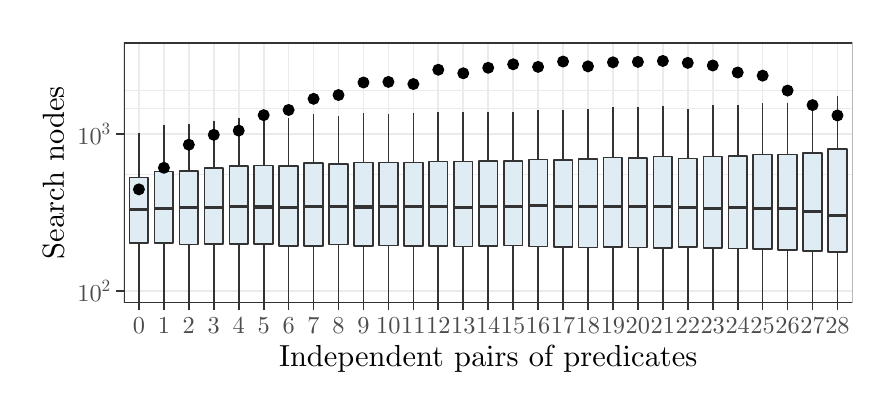
\begin{tikzpicture}[x=1pt,y=1pt]
\definecolor{fillColor}{RGB}{255,255,255}
\path[use as bounding box,fill=fillColor,fill opacity=0.00] (0,0) rectangle (303.53,130.09);
\begin{scope}
\path[clip] (  0.00,  0.00) rectangle (303.53,130.09);
\definecolor{drawColor}{RGB}{255,255,255}
\definecolor{fillColor}{RGB}{255,255,255}

\path[draw=drawColor,line width= 0.6pt,line join=round,line cap=round,fill=fillColor] (  0.00,  0.00) rectangle (303.53,130.09);
\end{scope}
\begin{scope}
\path[clip] ( 34.79, 30.69) rectangle (298.03,124.59);
\definecolor{fillColor}{RGB}{255,255,255}

\path[fill=fillColor] ( 34.79, 30.69) rectangle (298.03,124.59);
\definecolor{drawColor}{gray}{0.92}

\path[draw=drawColor,line width= 0.3pt,line join=round] ( 34.79, 77.01) --
	(298.03, 77.01);

\path[draw=drawColor,line width= 0.3pt,line join=round] ( 34.79,100.92) --
	(298.03,100.92);

\path[draw=drawColor,line width= 0.3pt,line join=round] ( 34.79,107.58) --
	(298.03,107.58);

\path[draw=drawColor,line width= 0.6pt,line join=round] ( 34.79, 34.95) --
	(298.03, 34.95);

\path[draw=drawColor,line width= 0.6pt,line join=round] ( 34.79, 91.75) --
	(298.03, 91.75);

\path[draw=drawColor,line width= 0.6pt,line join=round] ( 40.20, 30.69) --
	( 40.20,124.59);

\path[draw=drawColor,line width= 0.6pt,line join=round] ( 49.22, 30.69) --
	( 49.22,124.59);

\path[draw=drawColor,line width= 0.6pt,line join=round] ( 58.23, 30.69) --
	( 58.23,124.59);

\path[draw=drawColor,line width= 0.6pt,line join=round] ( 67.25, 30.69) --
	( 67.25,124.59);

\path[draw=drawColor,line width= 0.6pt,line join=round] ( 76.26, 30.69) --
	( 76.26,124.59);

\path[draw=drawColor,line width= 0.6pt,line join=round] ( 85.28, 30.69) --
	( 85.28,124.59);

\path[draw=drawColor,line width= 0.6pt,line join=round] ( 94.29, 30.69) --
	( 94.29,124.59);

\path[draw=drawColor,line width= 0.6pt,line join=round] (103.31, 30.69) --
	(103.31,124.59);

\path[draw=drawColor,line width= 0.6pt,line join=round] (112.32, 30.69) --
	(112.32,124.59);

\path[draw=drawColor,line width= 0.6pt,line join=round] (121.34, 30.69) --
	(121.34,124.59);

\path[draw=drawColor,line width= 0.6pt,line join=round] (130.35, 30.69) --
	(130.35,124.59);

\path[draw=drawColor,line width= 0.6pt,line join=round] (139.37, 30.69) --
	(139.37,124.59);

\path[draw=drawColor,line width= 0.6pt,line join=round] (148.38, 30.69) --
	(148.38,124.59);

\path[draw=drawColor,line width= 0.6pt,line join=round] (157.40, 30.69) --
	(157.40,124.59);

\path[draw=drawColor,line width= 0.6pt,line join=round] (166.41, 30.69) --
	(166.41,124.59);

\path[draw=drawColor,line width= 0.6pt,line join=round] (175.43, 30.69) --
	(175.43,124.59);

\path[draw=drawColor,line width= 0.6pt,line join=round] (184.44, 30.69) --
	(184.44,124.59);

\path[draw=drawColor,line width= 0.6pt,line join=round] (193.46, 30.69) --
	(193.46,124.59);

\path[draw=drawColor,line width= 0.6pt,line join=round] (202.47, 30.69) --
	(202.47,124.59);

\path[draw=drawColor,line width= 0.6pt,line join=round] (211.49, 30.69) --
	(211.49,124.59);

\path[draw=drawColor,line width= 0.6pt,line join=round] (220.50, 30.69) --
	(220.50,124.59);

\path[draw=drawColor,line width= 0.6pt,line join=round] (229.52, 30.69) --
	(229.52,124.59);

\path[draw=drawColor,line width= 0.6pt,line join=round] (238.53, 30.69) --
	(238.53,124.59);

\path[draw=drawColor,line width= 0.6pt,line join=round] (247.55, 30.69) --
	(247.55,124.59);

\path[draw=drawColor,line width= 0.6pt,line join=round] (256.56, 30.69) --
	(256.56,124.59);

\path[draw=drawColor,line width= 0.6pt,line join=round] (265.58, 30.69) --
	(265.58,124.59);

\path[draw=drawColor,line width= 0.6pt,line join=round] (274.59, 30.69) --
	(274.59,124.59);

\path[draw=drawColor,line width= 0.6pt,line join=round] (283.61, 30.69) --
	(283.61,124.59);

\path[draw=drawColor,line width= 0.6pt,line join=round] (292.62, 30.69) --
	(292.62,124.59);
\definecolor{drawColor}{gray}{0.20}

\path[draw=drawColor,line width= 0.6pt,line join=round] ( 40.20, 75.95) --
	( 40.20, 92.07);

\path[draw=drawColor,line width= 0.6pt,line join=round] ( 40.20, 52.30) --
	( 40.20, 43.78) --
	( 40.20, 30.65) --
	( 40.20,  0.76);
\definecolor{fillColor}{RGB}{224,236,244}

\path[draw=drawColor,line width= 0.6pt,line join=round,line cap=round,fill=fillColor] ( 36.82, 75.95) --
	( 36.82, 52.30) --
	( 40.20, 52.30) --
	( 43.58, 52.30) --
	( 43.58, 75.95) --
	( 40.20, 75.95) --
	( 36.82, 75.95) --
	cycle;

\path[draw=drawColor,line width= 1.1pt,line join=round] ( 36.82, 64.33) --
	( 40.20, 64.33) --
	( 43.58, 64.33);

\path[draw=drawColor,line width= 0.6pt,line join=round] ( 49.22, 78.10) --
	( 49.22, 94.85);

\path[draw=drawColor,line width= 0.6pt,line join=round] ( 49.22, 52.30) --
	( 49.22, 39.14) --
	( 49.22,  9.06);

\path[draw=drawColor,line width= 0.6pt,line join=round,line cap=round,fill=fillColor] ( 45.84, 78.10) --
	( 45.84, 52.30) --
	( 49.22, 52.30) --
	( 52.60, 52.30) --
	( 52.60, 78.10) --
	( 49.22, 78.10) --
	( 45.84, 78.10) --
	cycle;

\path[draw=drawColor,line width= 1.1pt,line join=round] ( 45.84, 64.78) --
	( 49.22, 64.78) --
	( 52.60, 64.78);

\path[draw=drawColor,line width= 0.6pt,line join=round] ( 58.23, 78.40) --
	( 58.23, 95.33);

\path[draw=drawColor,line width= 0.6pt,line join=round] ( 58.23, 51.68) --
	( 58.23, 37.75) --
	( 58.23,  2.66);

\path[draw=drawColor,line width= 0.6pt,line join=round,line cap=round,fill=fillColor] ( 54.85, 78.40) --
	( 54.85, 51.68) --
	( 58.23, 51.68) --
	( 61.61, 51.68) --
	( 61.61, 78.40) --
	( 58.23, 78.40) --
	( 54.85, 78.40) --
	cycle;

\path[draw=drawColor,line width= 1.1pt,line join=round] ( 54.85, 65.00) --
	( 58.23, 65.00) --
	( 61.61, 65.00);

\path[draw=drawColor,line width= 0.6pt,line join=round] ( 67.25, 79.27) --
	( 67.25, 96.45);

\path[draw=drawColor,line width= 0.6pt,line join=round] ( 67.25, 51.80) --
	( 67.25, 38.19) --
	( 67.25,  5.26);

\path[draw=drawColor,line width= 0.6pt,line join=round,line cap=round,fill=fillColor] ( 63.87, 79.27) --
	( 63.87, 51.80) --
	( 67.25, 51.80) --
	( 70.63, 51.80) --
	( 70.63, 79.27) --
	( 67.25, 79.27) --
	( 63.87, 79.27) --
	cycle;

\path[draw=drawColor,line width= 1.1pt,line join=round] ( 63.87, 65.00) --
	( 67.25, 65.00) --
	( 70.63, 65.00);

\path[draw=drawColor,line width= 0.6pt,line join=round] ( 76.26, 80.00) --
	( 76.26, 97.36);

\path[draw=drawColor,line width= 0.6pt,line join=round] ( 76.26, 51.80) --
	( 76.26, 38.19) --
	( 76.26,  5.26);

\path[draw=drawColor,line width= 0.6pt,line join=round,line cap=round,fill=fillColor] ( 72.88, 80.00) --
	( 72.88, 51.80) --
	( 76.26, 51.80) --
	( 79.64, 51.80) --
	( 79.64, 80.00) --
	( 76.26, 80.00) --
	( 72.88, 80.00) --
	cycle;

\path[draw=drawColor,line width= 1.1pt,line join=round] ( 72.88, 65.50) --
	( 76.26, 65.50) --
	( 79.64, 65.50);

\path[draw=drawColor,line width= 0.6pt,line join=round] ( 85.28, 80.28) --
	( 85.28, 97.67);

\path[draw=drawColor,line width= 0.6pt,line join=round] ( 85.28, 51.93) --
	( 85.28, 38.08) --
	( 85.28,  3.55);

\path[draw=drawColor,line width= 0.6pt,line join=round,line cap=round,fill=fillColor] ( 81.90, 80.28) --
	( 81.90, 51.93) --
	( 85.28, 51.93) --
	( 88.66, 51.93) --
	( 88.66, 80.28) --
	( 85.28, 80.28) --
	( 81.90, 80.28) --
	cycle;

\path[draw=drawColor,line width= 1.1pt,line join=round] ( 81.90, 65.29) --
	( 85.28, 65.29) --
	( 88.66, 65.29);

\path[draw=drawColor,line width= 0.6pt,line join=round] ( 94.29, 80.04) --
	( 94.29, 97.53);

\path[draw=drawColor,line width= 0.6pt,line join=round] ( 94.29, 51.30) --
	( 94.29, 37.75) --
	( 94.29,  5.26);

\path[draw=drawColor,line width= 0.6pt,line join=round,line cap=round,fill=fillColor] ( 90.91, 80.04) --
	( 90.91, 51.30) --
	( 94.29, 51.30) --
	( 97.67, 51.30) --
	( 97.67, 80.04) --
	( 94.29, 80.04) --
	( 90.91, 80.04) --
	cycle;

\path[draw=drawColor,line width= 1.1pt,line join=round] ( 90.91, 65.00) --
	( 94.29, 65.00) --
	( 97.67, 65.00);

\path[draw=drawColor,line width= 0.6pt,line join=round] (103.31, 81.09) --
	(103.31, 98.81);

\path[draw=drawColor,line width= 0.6pt,line join=round] (103.31, 51.30) --
	(103.31, 37.97) --
	(103.31,  6.85);

\path[draw=drawColor,line width= 0.6pt,line join=round,line cap=round,fill=fillColor] ( 99.93, 81.09) --
	( 99.93, 51.30) --
	(103.31, 51.30) --
	(106.69, 51.30) --
	(106.69, 81.09) --
	(103.31, 81.09) --
	( 99.93, 81.09) --
	cycle;

\path[draw=drawColor,line width= 1.1pt,line join=round] ( 99.93, 65.36) --
	(103.31, 65.36) --
	(106.69, 65.36);

\path[draw=drawColor,line width= 0.6pt,line join=round] (112.32, 80.74) --
	(112.32, 98.30);

\path[draw=drawColor,line width= 0.6pt,line join=round] (112.32, 51.68) --
	(112.32, 38.62) --
	(112.32,  9.06);

\path[draw=drawColor,line width= 0.6pt,line join=round,line cap=round,fill=fillColor] (108.94, 80.74) --
	(108.94, 51.68) --
	(112.32, 51.68) --
	(115.70, 51.68) --
	(115.70, 80.74) --
	(112.32, 80.74) --
	(108.94, 80.74) --
	cycle;

\path[draw=drawColor,line width= 1.1pt,line join=round] (108.94, 65.43) --
	(112.32, 65.43) --
	(115.70, 65.43);

\path[draw=drawColor,line width= 0.6pt,line join=round] (121.34, 81.32) --
	(121.34, 99.08);

\path[draw=drawColor,line width= 0.6pt,line join=round] (121.34, 51.30) --
	(121.34, 37.64) --
	(121.34,  4.42);

\path[draw=drawColor,line width= 0.6pt,line join=round,line cap=round,fill=fillColor] (117.96, 81.32) --
	(117.96, 51.30) --
	(121.34, 51.30) --
	(124.72, 51.30) --
	(124.72, 81.32) --
	(121.34, 81.32) --
	(117.96, 81.32) --
	cycle;

\path[draw=drawColor,line width= 1.1pt,line join=round] (117.96, 65.29) --
	(121.34, 65.29) --
	(124.72, 65.29);

\path[draw=drawColor,line width= 0.6pt,line join=round] (130.35, 81.32) --
	(130.35, 98.97);

\path[draw=drawColor,line width= 0.6pt,line join=round] (130.35, 51.43) --
	(130.35, 42.90) --
	(130.35, 29.76) --
	(130.35,  0.00);

\path[draw=drawColor,line width= 0.6pt,line join=round,line cap=round,fill=fillColor] (126.97, 81.32) --
	(126.97, 51.43) --
	(130.35, 51.43) --
	(133.73, 51.43) --
	(133.73, 81.32) --
	(130.35, 81.32) --
	(126.97, 81.32) --
	cycle;

\path[draw=drawColor,line width= 1.1pt,line join=round] (126.97, 65.64) --
	(130.35, 65.64) --
	(133.73, 65.64);

\path[draw=drawColor,line width= 0.6pt,line join=round] (139.37, 81.39) --
	(139.37, 99.17);

\path[draw=drawColor,line width= 0.6pt,line join=round] (139.37, 51.30) --
	(139.37, 37.97) --
	(139.37,  6.85);

\path[draw=drawColor,line width= 0.6pt,line join=round,line cap=round,fill=fillColor] (135.99, 81.39) --
	(135.99, 51.30) --
	(139.37, 51.30) --
	(142.75, 51.30) --
	(142.75, 81.39) --
	(139.37, 81.39) --
	(135.99, 81.39) --
	cycle;

\path[draw=drawColor,line width= 1.1pt,line join=round] (135.99, 65.64) --
	(139.37, 65.64) --
	(142.75, 65.64);

\path[draw=drawColor,line width= 0.6pt,line join=round] (148.38, 81.77) --
	(148.38, 99.66);

\path[draw=drawColor,line width= 0.6pt,line join=round] (148.38, 51.17) --
	(148.38, 37.53) --
	(148.38,  4.42);

\path[draw=drawColor,line width= 0.6pt,line join=round,line cap=round,fill=fillColor] (145.00, 81.77) --
	(145.00, 51.17) --
	(148.38, 51.17) --
	(151.76, 51.17) --
	(151.76, 81.77) --
	(148.38, 81.77) --
	(145.00, 81.77) --
	cycle;

\path[draw=drawColor,line width= 1.1pt,line join=round] (145.00, 65.43) --
	(148.38, 65.43) --
	(151.76, 65.43);

\path[draw=drawColor,line width= 0.6pt,line join=round] (157.40, 81.73) --
	(157.40, 99.63);

\path[draw=drawColor,line width= 0.6pt,line join=round] (157.40, 51.05) --
	(157.40, 37.64) --
	(157.40,  6.06);

\path[draw=drawColor,line width= 0.6pt,line join=round,line cap=round,fill=fillColor] (154.02, 81.73) --
	(154.02, 51.05) --
	(157.40, 51.05) --
	(160.78, 51.05) --
	(160.78, 81.73) --
	(157.40, 81.73) --
	(154.02, 81.73) --
	cycle;

\path[draw=drawColor,line width= 1.1pt,line join=round] (154.02, 65.14) --
	(157.40, 65.14) --
	(160.78, 65.14);

\path[draw=drawColor,line width= 0.6pt,line join=round] (166.41, 81.95) --
	(166.41, 99.79);

\path[draw=drawColor,line width= 0.6pt,line join=round] (166.41, 51.17) --
	(166.41, 37.97) --
	(166.41,  7.61);

\path[draw=drawColor,line width= 0.6pt,line join=round,line cap=round,fill=fillColor] (163.03, 81.95) --
	(163.03, 51.17) --
	(166.41, 51.17) --
	(169.79, 51.17) --
	(169.79, 81.95) --
	(166.41, 81.95) --
	(163.03, 81.95) --
	cycle;

\path[draw=drawColor,line width= 1.1pt,line join=round] (163.03, 65.43) --
	(166.41, 65.43) --
	(169.79, 65.43);

\path[draw=drawColor,line width= 0.6pt,line join=round] (175.43, 81.87) --
	(175.43, 99.71);

\path[draw=drawColor,line width= 0.6pt,line join=round] (175.43, 51.43) --
	(175.43, 38.19) --
	(175.43,  7.61);

\path[draw=drawColor,line width= 0.6pt,line join=round,line cap=round,fill=fillColor] (172.05, 81.87) --
	(172.05, 51.43) --
	(175.43, 51.43) --
	(178.81, 51.43) --
	(178.81, 81.87) --
	(175.43, 81.87) --
	(172.05, 81.87) --
	cycle;

\path[draw=drawColor,line width= 1.1pt,line join=round] (172.05, 65.64) --
	(175.43, 65.64) --
	(178.81, 65.64);

\path[draw=drawColor,line width= 0.6pt,line join=round] (184.44, 82.43) --
	(184.44,100.49);

\path[draw=drawColor,line width= 0.6pt,line join=round] (184.44, 51.05) --
	(184.44, 37.53) --
	(184.44,  5.26);

\path[draw=drawColor,line width= 0.6pt,line join=round,line cap=round,fill=fillColor] (181.06, 82.43) --
	(181.06, 51.05) --
	(184.44, 51.05) --
	(187.82, 51.05) --
	(187.82, 82.43) --
	(184.44, 82.43) --
	(181.06, 82.43) --
	cycle;

\path[draw=drawColor,line width= 1.1pt,line join=round] (181.06, 65.68) --
	(184.44, 65.68) --
	(187.82, 65.68);

\path[draw=drawColor,line width= 0.6pt,line join=round] (193.46, 82.36) --
	(193.46,100.38);

\path[draw=drawColor,line width= 0.6pt,line join=round] (193.46, 50.92) --
	(193.46, 37.97) --
	(193.46,  9.06);

\path[draw=drawColor,line width= 0.6pt,line join=round,line cap=round,fill=fillColor] (190.08, 82.36) --
	(190.08, 50.92) --
	(193.46, 50.92) --
	(196.84, 50.92) --
	(196.84, 82.36) --
	(193.46, 82.36) --
	(190.08, 82.36) --
	cycle;

\path[draw=drawColor,line width= 1.1pt,line join=round] (190.08, 65.43) --
	(193.46, 65.43) --
	(196.84, 65.43);

\path[draw=drawColor,line width= 0.6pt,line join=round] (202.47, 82.57) --
	(202.47,100.73);

\path[draw=drawColor,line width= 0.6pt,line join=round] (202.47, 50.66) --
	(202.47, 37.31) --
	(202.47,  6.06);

\path[draw=drawColor,line width= 0.6pt,line join=round,line cap=round,fill=fillColor] (199.09, 82.57) --
	(199.09, 50.66) --
	(202.47, 50.66) --
	(205.85, 50.66) --
	(205.85, 82.57) --
	(202.47, 82.57) --
	(199.09, 82.57) --
	cycle;

\path[draw=drawColor,line width= 1.1pt,line join=round] (199.09, 65.36) --
	(202.47, 65.36) --
	(205.85, 65.36);

\path[draw=drawColor,line width= 0.6pt,line join=round] (211.49, 83.13) --
	(211.49,101.31);

\path[draw=drawColor,line width= 0.6pt,line join=round] (211.49, 50.92) --
	(211.49, 37.53) --
	(211.49,  6.06);

\path[draw=drawColor,line width= 0.6pt,line join=round,line cap=round,fill=fillColor] (208.11, 83.13) --
	(208.11, 50.92) --
	(211.49, 50.92) --
	(214.87, 50.92) --
	(214.87, 83.13) --
	(211.49, 83.13) --
	(208.11, 83.13) --
	cycle;

\path[draw=drawColor,line width= 1.1pt,line join=round] (208.11, 65.50) --
	(211.49, 65.50) --
	(214.87, 65.50);

\path[draw=drawColor,line width= 0.6pt,line join=round] (220.50, 83.03) --
	(220.50,101.26);

\path[draw=drawColor,line width= 0.6pt,line join=round] (220.50, 50.66) --
	(220.50, 36.97) --
	(220.50,  3.55);

\path[draw=drawColor,line width= 0.6pt,line join=round,line cap=round,fill=fillColor] (217.12, 83.03) --
	(217.12, 50.66) --
	(220.50, 50.66) --
	(223.88, 50.66) --
	(223.88, 83.03) --
	(220.50, 83.03) --
	(217.12, 83.03) --
	cycle;

\path[draw=drawColor,line width= 1.1pt,line join=round] (217.12, 65.36) --
	(220.50, 65.36) --
	(223.88, 65.36);

\path[draw=drawColor,line width= 0.6pt,line join=round] (229.52, 83.55) --
	(229.52,101.89);

\path[draw=drawColor,line width= 0.6pt,line join=round] (229.52, 50.53) --
	(229.52, 36.97) --
	(229.52,  4.42);

\path[draw=drawColor,line width= 0.6pt,line join=round,line cap=round,fill=fillColor] (226.14, 83.55) --
	(226.14, 50.53) --
	(229.52, 50.53) --
	(232.90, 50.53) --
	(232.90, 83.55) --
	(229.52, 83.55) --
	(226.14, 83.55) --
	cycle;

\path[draw=drawColor,line width= 1.1pt,line join=round] (226.14, 65.36) --
	(229.52, 65.36) --
	(232.90, 65.36);

\path[draw=drawColor,line width= 0.6pt,line join=round] (238.53, 82.85) --
	(238.53,100.68);

\path[draw=drawColor,line width= 0.6pt,line join=round] (238.53, 50.79) --
	(238.53, 37.53) --
	(238.53,  6.85);

\path[draw=drawColor,line width= 0.6pt,line join=round,line cap=round,fill=fillColor] (235.15, 82.85) --
	(235.15, 50.79) --
	(238.53, 50.79) --
	(241.91, 50.79) --
	(241.91, 82.85) --
	(238.53, 82.85) --
	(235.15, 82.85) --
	cycle;

\path[draw=drawColor,line width= 1.1pt,line join=round] (235.15, 65.21) --
	(238.53, 65.21) --
	(241.91, 65.21);

\path[draw=drawColor,line width= 0.6pt,line join=round] (247.55, 83.58) --
	(247.55,101.97);

\path[draw=drawColor,line width= 0.6pt,line join=round] (247.55, 50.39) --
	(247.55, 37.08) --
	(247.55,  6.06);

\path[draw=drawColor,line width= 0.6pt,line join=round,line cap=round,fill=fillColor] (244.17, 83.58) --
	(244.17, 50.39) --
	(247.55, 50.39) --
	(250.93, 50.39) --
	(250.93, 83.58) --
	(247.55, 83.58) --
	(244.17, 83.58) --
	cycle;

\path[draw=drawColor,line width= 1.1pt,line join=round] (244.17, 64.78) --
	(247.55, 64.78) --
	(250.93, 64.78);

\path[draw=drawColor,line width= 0.6pt,line join=round] (256.56, 83.79) --
	(256.56,102.13);

\path[draw=drawColor,line width= 0.6pt,line join=round] (256.56, 50.26) --
	(256.56, 36.97) --
	(256.56,  6.06);

\path[draw=drawColor,line width= 0.6pt,line join=round,line cap=round,fill=fillColor] (253.18, 83.79) --
	(253.18, 72.33) --
	(253.18, 50.26) --
	(256.56, 50.26) --
	(259.94, 50.26) --
	(259.94, 72.33) --
	(259.94, 83.79) --
	(256.56, 83.79) --
	(253.18, 83.79) --
	cycle;

\path[draw=drawColor,line width= 1.1pt,line join=round] (253.18, 65.07) --
	(256.56, 65.07) --
	(259.94, 65.07);

\path[draw=drawColor,line width= 0.6pt,line join=round] (265.58, 84.22) --
	(265.58,102.80);

\path[draw=drawColor,line width= 0.6pt,line join=round] (265.58, 50.00) --
	(265.58, 37.31) --
	(265.58,  9.75);

\path[draw=drawColor,line width= 0.6pt,line join=round,line cap=round,fill=fillColor] (262.20, 84.22) --
	(262.20, 72.62) --
	(262.20, 50.00) --
	(265.58, 50.00) --
	(268.96, 50.00) --
	(268.96, 72.62) --
	(268.96, 84.22) --
	(265.58, 84.22) --
	(262.20, 84.22) --
	cycle;

\path[draw=drawColor,line width= 1.1pt,line join=round] (262.20, 64.78) --
	(265.58, 64.78) --
	(268.96, 64.78);

\path[draw=drawColor,line width= 0.6pt,line join=round] (274.59, 84.32) --
	(274.59,102.96);

\path[draw=drawColor,line width= 0.6pt,line join=round] (274.59, 49.73) --
	(274.59, 36.27) --
	(274.59,  4.42);

\path[draw=drawColor,line width= 0.6pt,line join=round,line cap=round,fill=fillColor] (271.21, 84.32) --
	(271.21, 72.65) --
	(271.21, 49.73) --
	(274.59, 49.73) --
	(277.98, 49.73) --
	(277.98, 72.65) --
	(277.98, 84.32) --
	(274.59, 84.32) --
	(271.21, 84.32) --
	cycle;

\path[draw=drawColor,line width= 1.1pt,line join=round] (271.21, 64.63) --
	(274.59, 64.63) --
	(277.98, 64.63);

\path[draw=drawColor,line width= 0.6pt,line join=round] (283.61, 84.89) --
	(283.61,103.68);

\path[draw=drawColor,line width= 0.6pt,line join=round] (283.61, 49.45) --
	(283.61, 36.39) --
	(283.61,  6.85);

\path[draw=drawColor,line width= 0.6pt,line join=round,line cap=round,fill=fillColor] (280.23, 84.89) --
	(280.23, 73.06) --
	(280.23, 49.45) --
	(283.61, 49.45) --
	(286.99, 49.45) --
	(286.99, 73.06) --
	(286.99, 84.89) --
	(283.61, 84.89) --
	(280.23, 84.89) --
	cycle;

\path[draw=drawColor,line width= 1.1pt,line join=round] (280.23, 63.57) --
	(283.61, 63.57) --
	(286.99, 63.57);

\path[draw=drawColor,line width= 0.6pt,line join=round] (292.62, 86.34) --
	(292.62,105.44);

\path[draw=drawColor,line width= 0.6pt,line join=round] (292.62, 49.04) --
	(292.62, 35.80) --
	(292.62,  5.26);

\path[draw=drawColor,line width= 0.6pt,line join=round,line cap=round,fill=fillColor] (289.24, 86.34) --
	(289.24, 74.16) --
	(289.24, 49.04) --
	(292.62, 49.04) --
	(296.01, 49.04) --
	(296.01, 74.16) --
	(296.01, 86.34) --
	(292.62, 86.34) --
	(289.24, 86.34) --
	cycle;

\path[draw=drawColor,line width= 1.1pt,line join=round] (289.24, 62.38) --
	(292.62, 62.38) --
	(296.01, 62.38);
\definecolor{drawColor}{RGB}{0,0,0}
\definecolor{fillColor}{RGB}{0,0,0}

\path[draw=drawColor,line width= 0.4pt,line join=round,line cap=round,fill=fillColor] ( 40.20, 71.66) circle (  1.96);

\path[draw=drawColor,line width= 0.4pt,line join=round,line cap=round,fill=fillColor] ( 49.22, 79.45) circle (  1.96);

\path[draw=drawColor,line width= 0.4pt,line join=round,line cap=round,fill=fillColor] ( 58.23, 87.80) circle (  1.96);

\path[draw=drawColor,line width= 0.4pt,line join=round,line cap=round,fill=fillColor] ( 67.25, 91.37) circle (  1.96);

\path[draw=drawColor,line width= 0.4pt,line join=round,line cap=round,fill=fillColor] ( 76.26, 92.89) circle (  1.96);

\path[draw=drawColor,line width= 0.4pt,line join=round,line cap=round,fill=fillColor] ( 85.28, 98.48) circle (  1.96);

\path[draw=drawColor,line width= 0.4pt,line join=round,line cap=round,fill=fillColor] ( 94.29,100.35) circle (  1.96);

\path[draw=drawColor,line width= 0.4pt,line join=round,line cap=round,fill=fillColor] (103.31,104.38) circle (  1.96);

\path[draw=drawColor,line width= 0.4pt,line join=round,line cap=round,fill=fillColor] (112.32,105.75) circle (  1.96);

\path[draw=drawColor,line width= 0.4pt,line join=round,line cap=round,fill=fillColor] (121.34,110.28) circle (  1.96);

\path[draw=drawColor,line width= 0.4pt,line join=round,line cap=round,fill=fillColor] (130.35,110.49) circle (  1.96);

\path[draw=drawColor,line width= 0.4pt,line join=round,line cap=round,fill=fillColor] (139.37,109.72) circle (  1.96);

\path[draw=drawColor,line width= 0.4pt,line join=round,line cap=round,fill=fillColor] (148.38,114.89) circle (  1.96);

\path[draw=drawColor,line width= 0.4pt,line join=round,line cap=round,fill=fillColor] (157.40,113.61) circle (  1.96);

\path[draw=drawColor,line width= 0.4pt,line join=round,line cap=round,fill=fillColor] (166.41,115.59) circle (  1.96);

\path[draw=drawColor,line width= 0.4pt,line join=round,line cap=round,fill=fillColor] (175.43,116.86) circle (  1.96);

\path[draw=drawColor,line width= 0.4pt,line join=round,line cap=round,fill=fillColor] (184.44,115.92) circle (  1.96);

\path[draw=drawColor,line width= 0.4pt,line join=round,line cap=round,fill=fillColor] (193.46,117.85) circle (  1.96);

\path[draw=drawColor,line width= 0.4pt,line join=round,line cap=round,fill=fillColor] (202.47,116.11) circle (  1.96);

\path[draw=drawColor,line width= 0.4pt,line join=round,line cap=round,fill=fillColor] (211.49,117.57) circle (  1.96);

\path[draw=drawColor,line width= 0.4pt,line join=round,line cap=round,fill=fillColor] (220.50,117.72) circle (  1.96);

\path[draw=drawColor,line width= 0.4pt,line join=round,line cap=round,fill=fillColor] (229.52,118.06) circle (  1.96);

\path[draw=drawColor,line width= 0.4pt,line join=round,line cap=round,fill=fillColor] (238.53,117.37) circle (  1.96);

\path[draw=drawColor,line width= 0.4pt,line join=round,line cap=round,fill=fillColor] (247.55,116.43) circle (  1.96);

\path[draw=drawColor,line width= 0.4pt,line join=round,line cap=round,fill=fillColor] (256.56,113.89) circle (  1.96);

\path[draw=drawColor,line width= 0.4pt,line join=round,line cap=round,fill=fillColor] (265.58,112.76) circle (  1.96);

\path[draw=drawColor,line width= 0.4pt,line join=round,line cap=round,fill=fillColor] (274.59,107.36) circle (  1.96);

\path[draw=drawColor,line width= 0.4pt,line join=round,line cap=round,fill=fillColor] (283.61,102.11) circle (  1.96);

\path[draw=drawColor,line width= 0.4pt,line join=round,line cap=round,fill=fillColor] (292.62, 98.37) circle (  1.96);
\definecolor{drawColor}{gray}{0.20}

\path[draw=drawColor,line width= 0.6pt,line join=round,line cap=round] ( 34.79, 30.69) rectangle (298.03,124.59);
\end{scope}
\begin{scope}
\path[clip] (  0.00,  0.00) rectangle (303.53,130.09);
\definecolor{drawColor}{gray}{0.30}

\node[text=drawColor,anchor=base west,inner sep=0pt, outer sep=0pt, scale=  0.88] at ( 17.96, 31.18) {10};

\node[text=drawColor,anchor=base west,inner sep=0pt, outer sep=0pt, scale=  0.62] at ( 26.76, 34.78) {2};

\node[text=drawColor,anchor=base west,inner sep=0pt, outer sep=0pt, scale=  0.88] at ( 17.96, 87.98) {10};

\node[text=drawColor,anchor=base west,inner sep=0pt, outer sep=0pt, scale=  0.62] at ( 26.76, 91.58) {3};
\end{scope}
\begin{scope}
\path[clip] (  0.00,  0.00) rectangle (303.53,130.09);
\definecolor{drawColor}{gray}{0.20}

\path[draw=drawColor,line width= 0.6pt,line join=round] ( 32.04, 34.95) --
	( 34.79, 34.95);

\path[draw=drawColor,line width= 0.6pt,line join=round] ( 32.04, 91.75) --
	( 34.79, 91.75);
\end{scope}
\begin{scope}
\path[clip] (  0.00,  0.00) rectangle (303.53,130.09);
\definecolor{drawColor}{gray}{0.20}

\path[draw=drawColor,line width= 0.6pt,line join=round] ( 40.20, 27.94) --
	( 40.20, 30.69);

\path[draw=drawColor,line width= 0.6pt,line join=round] ( 49.22, 27.94) --
	( 49.22, 30.69);

\path[draw=drawColor,line width= 0.6pt,line join=round] ( 58.23, 27.94) --
	( 58.23, 30.69);

\path[draw=drawColor,line width= 0.6pt,line join=round] ( 67.25, 27.94) --
	( 67.25, 30.69);

\path[draw=drawColor,line width= 0.6pt,line join=round] ( 76.26, 27.94) --
	( 76.26, 30.69);

\path[draw=drawColor,line width= 0.6pt,line join=round] ( 85.28, 27.94) --
	( 85.28, 30.69);

\path[draw=drawColor,line width= 0.6pt,line join=round] ( 94.29, 27.94) --
	( 94.29, 30.69);

\path[draw=drawColor,line width= 0.6pt,line join=round] (103.31, 27.94) --
	(103.31, 30.69);

\path[draw=drawColor,line width= 0.6pt,line join=round] (112.32, 27.94) --
	(112.32, 30.69);

\path[draw=drawColor,line width= 0.6pt,line join=round] (121.34, 27.94) --
	(121.34, 30.69);

\path[draw=drawColor,line width= 0.6pt,line join=round] (130.35, 27.94) --
	(130.35, 30.69);

\path[draw=drawColor,line width= 0.6pt,line join=round] (139.37, 27.94) --
	(139.37, 30.69);

\path[draw=drawColor,line width= 0.6pt,line join=round] (148.38, 27.94) --
	(148.38, 30.69);

\path[draw=drawColor,line width= 0.6pt,line join=round] (157.40, 27.94) --
	(157.40, 30.69);

\path[draw=drawColor,line width= 0.6pt,line join=round] (166.41, 27.94) --
	(166.41, 30.69);

\path[draw=drawColor,line width= 0.6pt,line join=round] (175.43, 27.94) --
	(175.43, 30.69);

\path[draw=drawColor,line width= 0.6pt,line join=round] (184.44, 27.94) --
	(184.44, 30.69);

\path[draw=drawColor,line width= 0.6pt,line join=round] (193.46, 27.94) --
	(193.46, 30.69);

\path[draw=drawColor,line width= 0.6pt,line join=round] (202.47, 27.94) --
	(202.47, 30.69);

\path[draw=drawColor,line width= 0.6pt,line join=round] (211.49, 27.94) --
	(211.49, 30.69);

\path[draw=drawColor,line width= 0.6pt,line join=round] (220.50, 27.94) --
	(220.50, 30.69);

\path[draw=drawColor,line width= 0.6pt,line join=round] (229.52, 27.94) --
	(229.52, 30.69);

\path[draw=drawColor,line width= 0.6pt,line join=round] (238.53, 27.94) --
	(238.53, 30.69);

\path[draw=drawColor,line width= 0.6pt,line join=round] (247.55, 27.94) --
	(247.55, 30.69);

\path[draw=drawColor,line width= 0.6pt,line join=round] (256.56, 27.94) --
	(256.56, 30.69);

\path[draw=drawColor,line width= 0.6pt,line join=round] (265.58, 27.94) --
	(265.58, 30.69);

\path[draw=drawColor,line width= 0.6pt,line join=round] (274.59, 27.94) --
	(274.59, 30.69);

\path[draw=drawColor,line width= 0.6pt,line join=round] (283.61, 27.94) --
	(283.61, 30.69);

\path[draw=drawColor,line width= 0.6pt,line join=round] (292.62, 27.94) --
	(292.62, 30.69);
\end{scope}
\begin{scope}
\path[clip] (  0.00,  0.00) rectangle (303.53,130.09);
\definecolor{drawColor}{gray}{0.30}

\node[text=drawColor,anchor=base,inner sep=0pt, outer sep=0pt, scale=  0.88] at ( 40.20, 19.68) {0};

\node[text=drawColor,anchor=base,inner sep=0pt, outer sep=0pt, scale=  0.88] at ( 49.22, 19.68) {1};

\node[text=drawColor,anchor=base,inner sep=0pt, outer sep=0pt, scale=  0.88] at ( 58.23, 19.68) {2};

\node[text=drawColor,anchor=base,inner sep=0pt, outer sep=0pt, scale=  0.88] at ( 67.25, 19.68) {3};

\node[text=drawColor,anchor=base,inner sep=0pt, outer sep=0pt, scale=  0.88] at ( 76.26, 19.68) {4};

\node[text=drawColor,anchor=base,inner sep=0pt, outer sep=0pt, scale=  0.88] at ( 85.28, 19.68) {5};

\node[text=drawColor,anchor=base,inner sep=0pt, outer sep=0pt, scale=  0.88] at ( 94.29, 19.68) {6};

\node[text=drawColor,anchor=base,inner sep=0pt, outer sep=0pt, scale=  0.88] at (103.31, 19.68) {7};

\node[text=drawColor,anchor=base,inner sep=0pt, outer sep=0pt, scale=  0.88] at (112.32, 19.68) {8};

\node[text=drawColor,anchor=base,inner sep=0pt, outer sep=0pt, scale=  0.88] at (121.34, 19.68) {9};

\node[text=drawColor,anchor=base,inner sep=0pt, outer sep=0pt, scale=  0.88] at (130.35, 19.68) {10};

\node[text=drawColor,anchor=base,inner sep=0pt, outer sep=0pt, scale=  0.88] at (139.37, 19.68) {11};

\node[text=drawColor,anchor=base,inner sep=0pt, outer sep=0pt, scale=  0.88] at (148.38, 19.68) {12};

\node[text=drawColor,anchor=base,inner sep=0pt, outer sep=0pt, scale=  0.88] at (157.40, 19.68) {13};

\node[text=drawColor,anchor=base,inner sep=0pt, outer sep=0pt, scale=  0.88] at (166.41, 19.68) {14};

\node[text=drawColor,anchor=base,inner sep=0pt, outer sep=0pt, scale=  0.88] at (175.43, 19.68) {15};

\node[text=drawColor,anchor=base,inner sep=0pt, outer sep=0pt, scale=  0.88] at (184.44, 19.68) {16};

\node[text=drawColor,anchor=base,inner sep=0pt, outer sep=0pt, scale=  0.88] at (193.46, 19.68) {17};

\node[text=drawColor,anchor=base,inner sep=0pt, outer sep=0pt, scale=  0.88] at (202.47, 19.68) {18};

\node[text=drawColor,anchor=base,inner sep=0pt, outer sep=0pt, scale=  0.88] at (211.49, 19.68) {19};

\node[text=drawColor,anchor=base,inner sep=0pt, outer sep=0pt, scale=  0.88] at (220.50, 19.68) {20};

\node[text=drawColor,anchor=base,inner sep=0pt, outer sep=0pt, scale=  0.88] at (229.52, 19.68) {21};

\node[text=drawColor,anchor=base,inner sep=0pt, outer sep=0pt, scale=  0.88] at (238.53, 19.68) {22};

\node[text=drawColor,anchor=base,inner sep=0pt, outer sep=0pt, scale=  0.88] at (247.55, 19.68) {23};

\node[text=drawColor,anchor=base,inner sep=0pt, outer sep=0pt, scale=  0.88] at (256.56, 19.68) {24};

\node[text=drawColor,anchor=base,inner sep=0pt, outer sep=0pt, scale=  0.88] at (265.58, 19.68) {25};

\node[text=drawColor,anchor=base,inner sep=0pt, outer sep=0pt, scale=  0.88] at (274.59, 19.68) {26};

\node[text=drawColor,anchor=base,inner sep=0pt, outer sep=0pt, scale=  0.88] at (283.61, 19.68) {27};

\node[text=drawColor,anchor=base,inner sep=0pt, outer sep=0pt, scale=  0.88] at (292.62, 19.68) {28};
\end{scope}
\begin{scope}
\path[clip] (  0.00,  0.00) rectangle (303.53,130.09);
\definecolor{drawColor}{RGB}{0,0,0}

\node[text=drawColor,anchor=base,inner sep=0pt, outer sep=0pt, scale=  1.10] at (166.41,  7.64) {Independent pairs of predicates};
\end{scope}
\begin{scope}
\path[clip] (  0.00,  0.00) rectangle (303.53,130.09);
\definecolor{drawColor}{RGB}{0,0,0}

\node[text=drawColor,rotate= 90.00,anchor=base,inner sep=0pt, outer sep=0pt, scale=  1.10] at ( 13.08, 77.64) {Search nodes};
\end{scope}
\end{tikzpicture}

\end{document}

  \caption{The distribution of the number of nodes in the binary search tree as
    a function of the number of independent pairs of predicates for
    $|\predicates| = 8$. Significant outliers are hidden, the dots denote mean
    values, and the vertical axis is on a $\log_{10}$ scale.}
  \label{fig:phase_transition}
\end{figure*}

Along with constraints, variables, and their domains, two more design decisions
are needed to complete the model: heuristics and restarts. By trial and error,
the variable ordering heuristic was devised to eliminate sources of thrashing,
i.e., situations where a contradiction is being `fixed' by making changes that
have no hope to fix the contradiction. Thus, we partition all decision variables
into an ordered list of groups, and require the values of all variables from one
group to be determined before moving to the next group. Within each group, we
use the `fail first' variable ordering heuristic. The first group consists of
all head predicates. Afterwards, we handle all remaining decision variables from
the first clause before proceeding to the next. The decision variables within
each clause are divided into:
\begin{enumerate*}
\item the $\variable{structure}$ array,
\item body predicates,
\item head arguments,
\item (if $|\variables{}| > 1$) the $\variable{intros}$ array,
\item body arguments.
\end{enumerate*}
For instance, in the clause from \cref{example:sibling}, all visible parts of
the clause would be decided in this order:
\[
  \overset{1}{\mathsf{sibling}}(\overset{3}{X}, \overset{3}{Y}) \gets
  \overset{2}{\mathsf{parent}}(\overset{4}{X}, \overset{4}{Z})
  \overset{2}{\land} \overset{2}{\mathsf{parent}}(\overset{4}{Y},
  \overset{4}{Z}).
\]
We also employ a geometric restart policy, restarting after $10, 20, 40,
80, \dots$ contradictions.

We ran close to \num{400000} experiments, investigating whether the model is
efficient enough to generate reasonably-sized programs and gaining insight into
what parameter values make the constraint satisfaction problem harder. For these
experiments, we use Choco~4.10.2 \citep{choco} with Java~8 on a personal
computer with an Intel Core i5-8250U processor and Arch Linux 5.4.12-arch1-1
operating system. For $|\predicates{}|$, $|\variables{}|$, $|\constants{}|$,
$\maxNumNodes{}$, and $\maxNumClauses{} - |\predicates{}|$ (i.e., the number of
clauses in addition to the mandatory $|\predicates{}|$ clauses), we assign all
combinations of 1, 2, 4, 8. $\maxArity{}$ is assigned to values 1--4. For each
$|\predicates{}|$, we also iterate over all possible numbers of independent
pairs of predicates, ranging from 0 up to $\binom{|\predicates{}|}{2}$. For each
combination of the above-mentioned parameters, we pick ten random pairs of:
$\arities{}$ (such that $\maxArity{}$ occurs at least once) and the required
number of independent pairs (without repetition). We then run the solver with a
\SI{60}{\second} timeout.

The vast majority (\SI{97.7}{\percent}) of runs finished in under
\SI{1}{\second}, while four instances timed out: all with $|\predicates| =
\maxNumClauses{} - |\predicates{}| = \maxNumNodes{} = 8$ and the remaining
parameters all different. This suggests that---regardless of parameter
values---most of the time a solution can be identified instantaneously while
occasionally a series of wrong decisions can lead the solver into a part of the
search space with no solutions.

In \cref{fig:impact}, we plot how the mean number of nodes in the binary search
tree grows as a function of each parameter (the plot for the median is very
similar). The growth of each curve suggest how well/poorly the model scales with
higher values of the parameter. From this plot, it is clear that
$\maxNumNodes{}$ is the limiting factor. This is because some tree structures
can be impossible to fill with predicates without creating either a negative
cycle or a forbidden dependence, and such trees become more common as the number
of nodes increases.

\cref{fig:phase_transition} takes the data for $|\predicates{}| = 8$ (almost
\num{300000} observations) and shows how the number of nodes in the search tree
varies with the number of independent pairs of predicates. The box plots show
that the median number of nodes stays about the same while the dots
(representing the means) draw an arc. This suggests a type of phase transition,
but only in mean rather than median, i.e., most problems remain easy, but with
some parameter values hard problems become more likely. On the one hand, with
few pairs of independent predicates, one can easily find the right combination
of predicates to use in each clause. On the other hand, if most predicates must
be independent, this leaves fewer predicates that can be used in the body of
each clause (since all of them have to be independent with the head predicate),
and we can either quickly find a solution or identify that there is none.

% TODO: talk about randomness. The value heuristic is random because we want
% randomness. After finding one solution, one can continue the search for more,
% but they will be similar (acceptable if the search space is small and we want
% to find all solutions).

\section{CONCLUSION \& FUTURE WORK}

\begin{itemize}
\item A constraint for logical equivalence. An algorithm to reduce each tree to
  some kind of normal form. Not doing this on purpose. Leaving for further work.
\item Could investigate how uniform the generated distribution of programs is.
  Distributions of individual parameters will often favour larger values
  because, e.g., there are more 5-tuples than 4-tuples.
%\item Inference options to explore. Logspace vs normal space. Symbolic vs
%  non-symbolic. Propagate evidence (might be irrelevant)? Propagate weights?
%  Supported knowledge compilation techniques: sdd, sddx, bdd, nnf, ddnnf, kbest,
%  fsdd, fbdd.
\item Mention the random heuristic. Mention that restarting gives better
  randomness, but duplicates become possible.
\item Could add statistics about what constraints tend to conflict.
\end{itemize}

\subsubsection*{Acknowledgements}

% The author would like to thank Vaishak Belle for his comments.
This work was supported by the EPSRC Centre for Doctoral Training in Robotics
and Autonomous Systems, funded by the UK Engineering and Physical Sciences
Research Council (grant EP/S023208/1).

\renewcommand{\bibsection}{\subsubsection*{References}}
\bibliography{paper}
\end{document}
